\begin{savequote}[75mm] 
Our posturings, our imagined self-importance, the delusion that we have some privileged position in the Universe, are challenged by this point of pale light.
\qauthor{Carl Sagan, Pale Blue Dot, 1994} 
\end{savequote}

\chapter{Visualization in Bioinformatics} \label{section:visualization}




\begin{description}
	\item[First author publications]:\\
		\begin{enumerate}
			\item \label{paper:PPI} \bibentry{SAL2014}
			\item  \label{paper:PINV} \bibentry{SAL2014pinv}
%			\item Gustavo A. Salazar et al. \emph{PPI layouts: BioJS components for the display of Protein-Protein Interactions} in  \emph{F1000Research} 2014, 3:50 (doi: 10.12688/f1000research.3-50.v1) [v1; ref status: indexed, http://f1000r.es/2u5]
%			\item Gustavo A. Salazar et al. \emph{A web-based protein interaction network visualizer} In \emph{BMC Bioinformatics} 2014, 15:129  doi:10.1186/1471-2105-15-129
		\end{enumerate}

	\item[Coauthor publications]:\\
		\begin{enumerate}
			\setcounter{enumi}{2}
			\item \label{paper:biojs1} \bibentry{GOM2013}
			\item \label{paper:biojs2} \bibentry{COR2014}
%			\item John Gomez et al. \emph{BioJS: an open source JavaScript framework for biological data visualization} in  \emph{Bioinformatics}  2013 29 (8): 1103-1104. doi: 10.1093/bioinformatics/btt100
%			\item Manuel Corpas et al. \emph{BioJS: an open source standard for biological visualisation – its status in 2014} In \emph{F1000Research} 2014, 3:55 (doi: 10.12688/f1000research.3-55.v1)  [v1; ref status: indexed, http://f1000r.es/2yy]
		\end{enumerate}
 
	\item[Author's Contibutions]:\\
		\begin{enumerate}
			\item Critical revision of the manuscript for important intellectual input: GS, AM and NM. Supervision: NM. Study concept: GS, AM and NM. Software development: GS. Drafting of the manuscript: GS and AM. All authors have read and approved the final manuscript.
			\item Critical revision of the manuscript for important intellectual input: GS, AM, GM, HR, RA and NM. Study concept: GS, AM and NM. Software Design: GS, AM, GM, HR, RA and NM. Software development: GS and AM. Creation of datasets: GM, HR and RA. Software Testing: GM, HR, RA and NM. Software Documentation: GS and RA. Drafting of the manuscript: GS, HR and NM. Supervision: NM. All authors read and approved the final manuscript;
			\item All authors have participated in the development of the BioJS community through provision of code, meeting attendance or writing of grants.
			\item All authors have participated in the development of the BioJS community through provision of code, meeting attendance or writing of grants.
		\end{enumerate}
\end{description}
\newpage
\newthought{A single point in a photograph can represent our whole known world}, as shown in the famous image acquired by the Voyager 1 spacecraft in 1990. From that perspective, is impossible to perceive all details that conform our planet, from rivers to highways, from mountains to buildings, even countries or full continents and oceans are undistinguished in the mentioned picture. Nonetheless, the image gave us a insight of the vastness of the universe in comparison with our known world.

As in the previous example the same object can be seen from different perspectives. Each of them can highlight some features and hide others, hence the importance of choosing the right representation for the object in display.

This chapter describes the contributions that are the object of this PhD project on the visualisation of bioinformatics data. We first described BioJS, a community project to create a library of bioinformatics web components, including some widgets that we have been developed to be part of the library. The second part of this chapter focuses on PINV, a tool to visualise PPI networks using web technologies.


\section{BioJS: A JavaScript framework for Biological Web 2.0 Applications }
We participated in the community effort to create a specification and develop an standard for web components in Javascript, called BioJavaScript, or BioJS for short. BioJS has been described in the publications \ref{paper:biojs1} and \ref{paper:biojs2} listed at the beginning of this chapter. We believe relevant to include a description about BioJS, not only because of our contribution to it, but also because we have followed the proposed standard for the creation of a set of visualisation components described in the section \ref{subsec:biojs_components}. Some of those components were used to create the web based tool PINV, described in section \ref{section:pinv}.

We want to explicitly express that by including this description here we are not taking credit of the development of BioJS. BioJS is the result of a group effort and has many contributors, most of which are listed here \url{http://biojs.net/biojs_team.html}. Our contribution to the project has been in the form of software, documentation and participating in multiple project meetings.

BioJS is an open-source and community-driven project that aims to provide a framework to facilitate the reutilisation of JavaScript components for the visualisation of biological data in the web \cite{GOM2013}. At the hearth of BioJS 1.0 is a registry of components (\url{http://www.ebi.ac.uk/Tools/biojs/registry/index.html}) in which developers following the BioJS guidelines can publish their components; and simultaneously creators of web content for biological tools, can find the right visualisation widget for their purposes.

The project started at the EBI in 2011 and its first version was officially released when the first publication about the project was written \cite{GOM2013}. By then, the registry had 29 component registered, thanks to an effort from all the collaborators in order to count with a heterogeneous set of tools available for this release.

In the first version a BioJS component should follow the object oriented paradigm and inherit from a common class called BioJS. In this class certain routines were implemented in order to ensure a common behaviour in between the components. The most important things included in this class were: an event manager, an object creation subroutine, an standard way to receive parameters and a group of utility functions.

An example of how several BioJS components can interact is shown in the right side of figure \ref{fig:biojs_layers}. The secondary structure of a protein (bottom-left) can be displayed when the protein is selected from a PPI network (top), and a region on the 3D structured (bottom-right) can be highlighted, when the mouse hovers on one of the substructures of the bottom-left component.

BioJS components are flexible enough to manipulate web elements for visualisations: SVG, Canvas, CSS, and in general anything that can be controlled via Javascript. BioJS is framework agnostic, allowing each component to define its own dependencies. This schema supports the interaction of two or more components that have been implemented using different JavaScript frameworks (e.g. JQuery, YUI, Prototype, etc.).
 
Another aspect defined in BioJS 1.0 was the use of JSDoc to include in-code comments, this code was not only use to create the usual reference documentation, but it was key in the generation of the running examples of the components in the registry. 

The developer was requested to include snippets of its code and a list of the dependencies as part of the documentation.That information is used to generate the pages in the registry that include a running example, instructions on how to include the dependencies, and all the generated documentation for methods, events and parameters.

\begin{figure}  
\centering
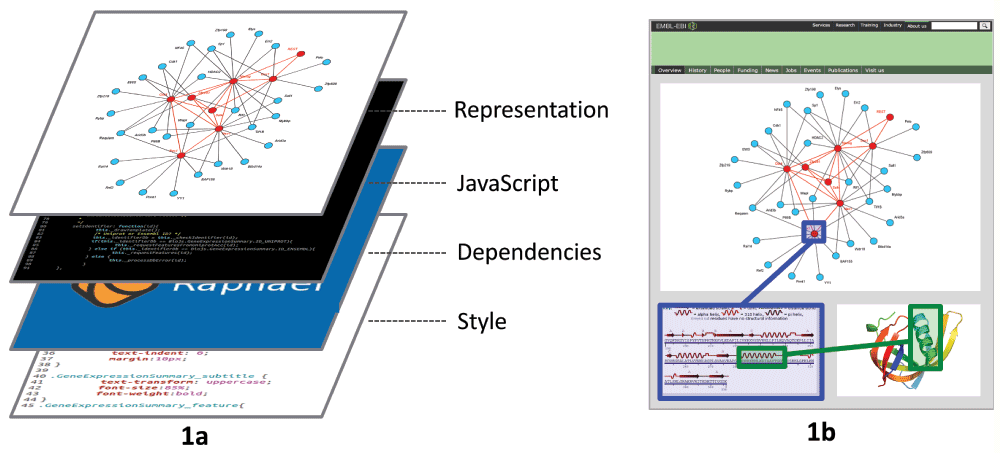
\includegraphics[width=\textwidth]{figures/biojs_layers.png}
\caption[BioJS layers.]{1a shows the different layers that a BioJS component is divided into. The representation layer sits on top of the JavaScript layer, which similarly possesses a layer of dependencies and a style. 1b presents an example of interactivity between three components, a protein-protein interaction network viewer, a secondary structure viewer and a tertiary structure viewer. 
\label{fig:biojs_layers}}
\end{figure}
 
The layer separation in the BioJS architecture is shown in the left side of figure \ref{fig:biojs_layers}. The final representation of a component can be deployed in any of the different methods supported in web, the control of such representation is programmed in JavaScript, supported by any of the libraries the developer choose to have as dependencies. If the chosen representation is based on HTML standards, all its elements can be stylised via Cascade Style Sheets CSS \cite{COR2014}.

Here are some examples of different methods to represent data in web with examples of BioJS components using them.
\begin{description}
\setlength\itemsep{-0.3em}
\item[HTML documents] Where HTML is generated to display data, for instance \emph{Biojs.InteractionsTable} (\url{http://www.ebi.ac.uk/Tools/biojs/registry/Biojs.InteractionsTable.html}) creates a HTML table that contains information about protein interactions (Figure \ref{fig:biojs_components} a).
\item[Visualizations using HTML elements] Similar to the previous one, but the HTML generated is organise in certain way to represent the data. For example,  \emph{Biojs.Chromosome} (\url{http://www.ebi.ac.uk/Tools/biojs/registry/Biojs.Chromosome.html}) uses the div HTML element to create boxes representing the bands of a chromosome (Figure \ref{fig:biojs_components} b).
\item[Scalable Vector Graphics] HTML supports the SVG format, and because SVG is a Markup language, its manipulation is similar to when dealing with HTML content. The \emph{Biojs.FeatureViewer} (\url{http://www.ebi.ac.uk/Tools/biojs/registry/Biojs.FeatureViewer.html}) uses this technique to display protein annotations (Figure \ref{fig:biojs_components} c).
\item[HTML canvas] Since HTML5 the element canvas is part of the specification, this component provides a programatic way to generate graphics. It is faster than SVG, but doesn't offer as much control on each of the drawn elements. For example, a representation of the metabolic pathways provided by KEGG is displayed by the \emph{Biojs.KEGGViewer} (\url{http://www.ebi.ac.uk/Tools/biojs/registry/Biojs.KEGGViewer.html}) component using the canvas element (Figure \ref{fig:biojs_components} d).
\item[Browser plugins] The use of third party tools such as Java Applets or Adobe Flash objects is also possible as long an interface with JavaScript is provided, for example \emph{Biojs.Protein3D} (\url{http://www.ebi.ac.uk/Tools/biojs/registry/Biojs.Protein3D.html}) displays the 3D structure of a proteins by using the JMol Java applet (Figure \ref{fig:biojs_components} e).
\end{description}

Besides the diversity in the chosen technology to represent the data, figure \ref{fig:biojs_components} also shows the variety of visualisation techniques that can be implemented using BioJS, from text tables to 3D objects.

\begin{figure}  
\centering
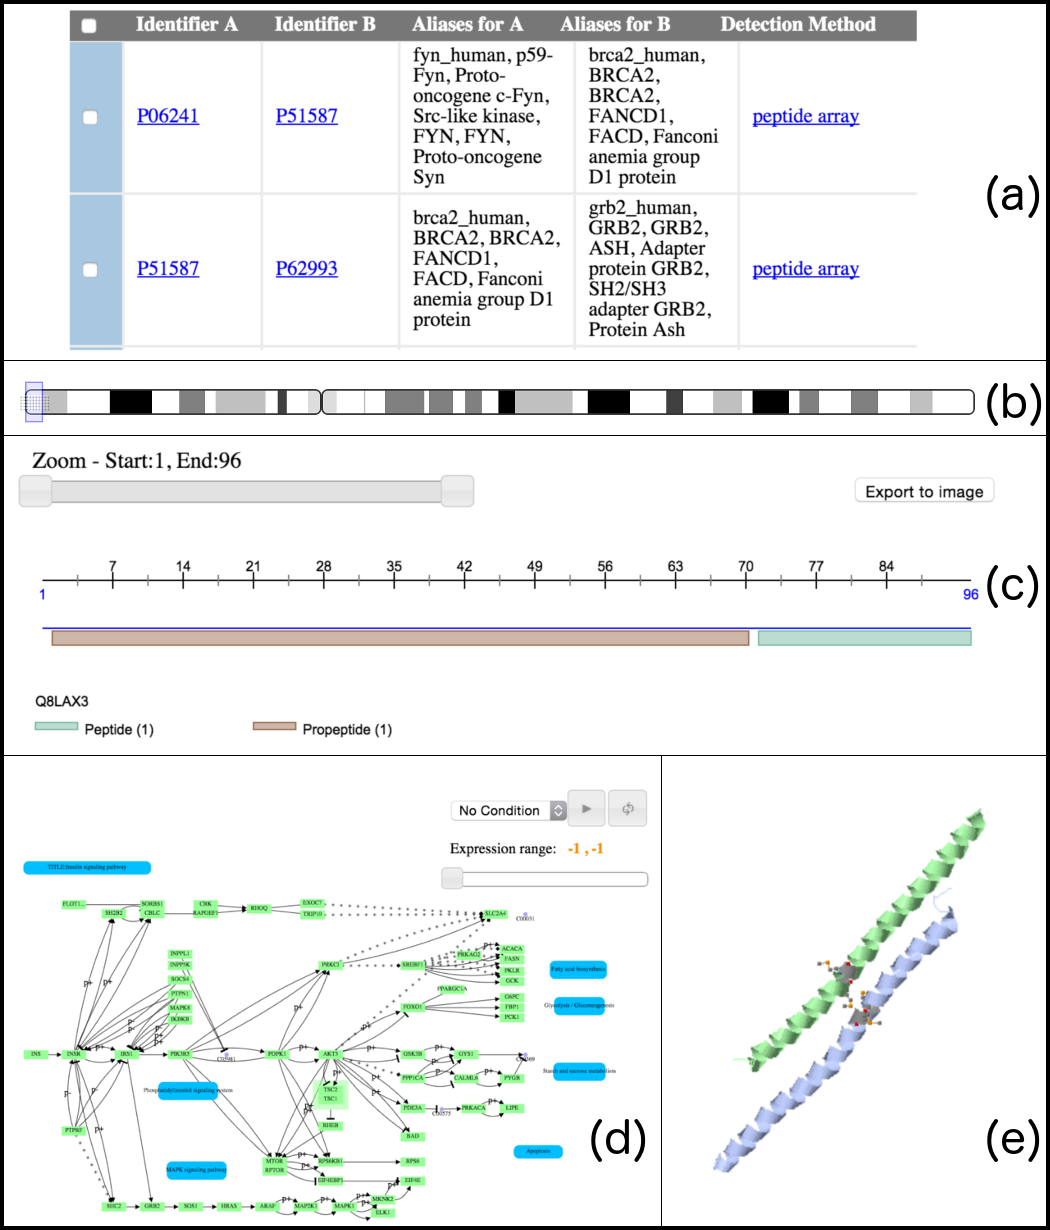
\includegraphics[width=\textwidth]{figures/biojs_components.png}
\caption[Snapshots of some BioJS components.]{Snapshots of some BioJS components. (a) Biojs.InteractionsTable, (b) Biojs.Chromosome, (c) Biojs.FeatureViewer, (d) Biojs.KEGGViewer and  (e) Biojs.Protein3D.
\label{fig:biojs_components}}
\end{figure}
 


BioJS ambitious vision is ``\emph{that every online biological dataset in the world should be visualised with BioJS tools}''. In order to accomplish it, BioJS requires to provide a convenient environment for the different roles related to the visualisation of biological data. The roles that we have identified are: data providers,  developers of web components, developers using ready-to-use components and the users that finally visit web tools that include those components.

A data provider can benefit from BioJS by simply reusing existing components that can visualise their type of data, and in this way save the resources that a development form scratch requires. Even if there is not component that fully covers the needs of the institution, is likely that there is a component that provide a partial solution, and thanks that BioJS an open-source project, the institution can extend the existing component, improving its feature set, or create an alternative version of it tailoring to the needs of the institution. In the case where the required representation is so unique, that the institution requires to develop the component from scratch, they still get the benefit of ensuring that anyone else who will display their data, will count with a widget that visualise it exactly in the way they intended to do so. The two last cases ultimately reflect in growth over the BioJS library for the benefit of other BioJS actors.

Developers creating new visualisations with BioJS can get exposure and acknowledgements for their efforts. Their widgets will be now visible in an open forum, where a community of potential users and collaborators can both, benefit and contribute to the improvement of the widget. On the technical side, a developer following the BioJS guidelines is not limited by any dependency, and although the need of writing documentation and applying a code structure, implies more time on the creation of the resource, it also ensures the robustness of the components.

When a developer wants to include a component to display some type of biological data, they can take advantage of BioJS by easily follow the common installation instructions provided in the registry, which have been customised for each of the components. The registry supports navigation and search of components, but we consider the bigger benefit for developers is to be able to run live demos of the components and the code to generate them. In this way, someone interested in a widget can seen it in action, without having to install or develop anything.

All of it has as the final beneficiary the researcher, who ultimately is the one who will interact with the different components getting a dynamic view of the data in the way the provider expected, in a component that can be improved by a community of visualisation experts, and has been chosen to be in the web tool that the user is visiting because it is the one that highlights the features of the data in the best way.

We are aware that this is still a work in progress, but the results so far obtained from the project are very positive. For example, the journal F1000research decided to publish an special collection of articles describing BioJS component. We have discussed before our opinion about how positive is for projects to provide an environment for the publication of peer-reviwed articles (Section \ref{subsubsec:ppi_biojs}). We consider that this collection of BioJS articles is an important step in the right path for the growth of the project and its contributions to the research community. The section \ref{subsubsec:ppi_biojs} describes the details of an article included in this collection, in which BioJS components for the visualisation of PPI networks are introduced.

\subsection{BioJS 2.0}
Besides the relative success of the first version of BioJS, its community identified a number of deficiencies and areas where the project can be improved. For example after BioJS first version was released, the focus of the community was directed to new components, and for around 3 years the core did not change much. During that time some of the libraries and strategies used got outdated, for example, the registry required compilation using maven (\url{http://maven.apache.org/}) in order to generate the web content for each of the components. This seemed a good idea at the beginning of the project, however became a problem because of the delay in the publication of components, and more importantly the lack of a protocol to retrieve the dependencies of each components.

The registry was still bringing visibility to the components, but it was failing to attract developers to create new widgets using the proposed guidelines. This was the main motivation to work on BioJS 2.0.

A concentrated effort looking to push forward the new version of BioJS was held during the 4th and 6th of August of 2014. The event was hosted in Munich Germany (\url{http://biojs.net/code/2014/07/04/announcing-hackathon.html}) and it was also possible to collaborate remotely. 

The motto of this event was to bring ``easiness'' back to BioJS. This principle has transcend from the event to become the goal of BioJS 2.0.  The efforts were mainly made from the point of view of the developer of new components: BioJS should be easy to develop, maintain and test, which should be done without failing to offer the benefits to the other BioJS stake holders and therefore BioJS should continue to be easy to use, combine and discover.

The main strategy to be able to provide the desired ``easiness'' was to give freedom to the developer, which in BioJS terms meant to deprecate the predefined class where all the components used to inherit, it also implied to abolish the requirement to follow the JSDoc format to document and introduce easily editable, working examples of an component and moving the documentation to a public README file or any other form chosen by the developer (e.g. github wiki).

The alternative was to define a set of guidelines called ``the gold standard" (\url{http://edu.biojs.net/series/102/70_gold_standard.html}). It includes recommendations on how to test, document, publish and create examples for a BioJS component. The key behind these recommendations is that all of them are supported by web resources that can be accessed programatically. The registry is then able to detect when a recommendation is followed by a component, and present this information to users exploring the components. For example, the sniper package (\url{https://github.com/biojs/sniper}) facilitates the inclusion of live examples in the component's page.

This implementation in the registry was done by extensively use two well know development resources available in the web: The web-based Git repository hosting service: GitHub; and the node package manager (npm). 

All the code of BioJS was migrated to the source control system git (\url{http://git-scm.com/}) and the repositories are hosted by GitHub (\url{https://github.com/biojs/}). The source code of the components is now independently manage by their authors, and the only components in the BioJS repository are the ones related with the core functions, such as the registry or helpers to follow the gold standard.

A developer creating a BioJS component should publish its code as a npm package (\url{https://www.npmjs.com/}). npm is in itself a registry of packages for javascript components, which has programmatic access from a command line client, but also can be browsed using its online front end (\url{https://www.npmjs.com}). All the configuration and metadata of a npm package should be included in a file named package.json, which should be located at root of the package folder. BioJS builds upon this standards and added custom fields for meta information to the package.json file.

%One of the reasons why npm has been chosen as a base technology for BioJS is the way it manages the dependencies of a package: when a npm package is installed all its dependencies are automatically downloaded, including recursive ones (i.e. when a dependency has dependencies). In this way BioJS 2.0 solves what was a big issue of its previous version. 

By February 2015 npm had more than 120000 packages in its repository, with an extraordinary growth rate of 221 packages per day, as reported by the independent website \url{http://www.modulecounts.com/}. The high adoption of the npm repository is an advantage for BioJS developers because it provides an extensive tool set to work with, which scope goes beyond the visualisation of biological data.

With this model, the developer is now free to use any package to accomplish any of the BioJS guidelines, and as long it is reported in the package.json file it can be reported in the BioJS registry. The reporting of the gold standard implemented features it is still a work in progress, nonetheless a fully operational registry for BioJS2.0 is available at \url{http://biojs.io/}.

It is important to highlight the continuous effort from the BIoJS community to provide up to date documentation . The web portal \url{http://edu.biojs.net/} contains tutorials and reference documents to help the developers of new BioJS components.

\begin{figure}  
\centering
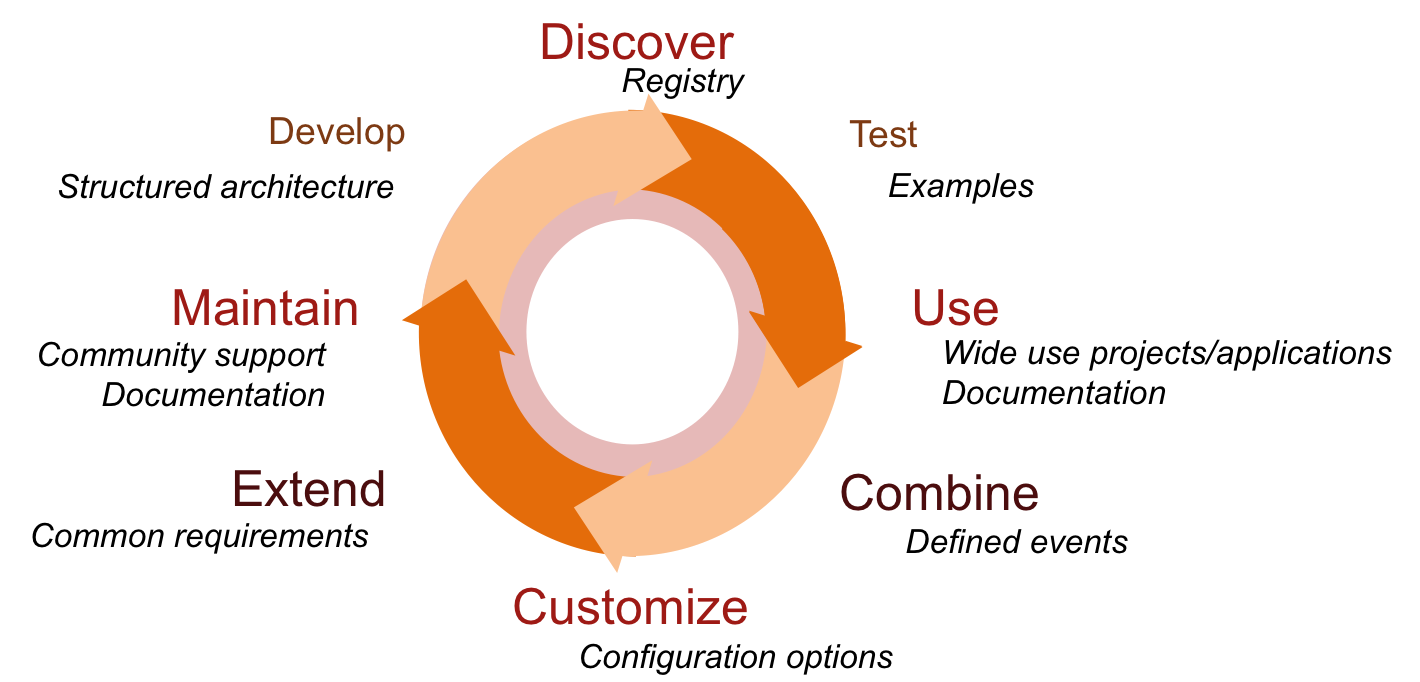
\includegraphics[width=\textwidth]{figures/biojs_cycle.png}
\caption[Cycle of a BioJS component]{Cycle of a BioJS component.
\label{fig:biojs_cycle}}
\end{figure}

Figure \ref{fig:biojs_cycle} represents the development stages of  a BioJS component, below we describe some of the technical details on how BioJS 2.0 assists in each of these stages.

\subsubsection{Develop}
The developer is free to use any javascript framework or visualisation library as a dependency. the only requirement is to report them in the package.json file. Ideally the dependencies should also be npm packages, in order to support recursive checking. However is also possible to include required files as part of the package. 

There is an assistant package to generate a template for a BioJS project (\url{http://biojs.io/d/slush-biojs}). The package was created using Slush(\url{https://slushjs.github.io}) and once executed, it includes some dependencies and configurations useful to comply some of the guidelines in the BioJS gold standard.

\subsubsection{Discover}
The only requirement for a npm package to be included in the BioJS 2.0 repository is to contain the tag ``\emph{biojs}'' in the package.json file. The BioJS registry queries npm to check for published packages with the ``\emph{biojs}'' tag and processes their configuration files in order to extract all the information about documentation, tests, etc.% and to dynamically generate with it, the content that other users will find about this component.

%The registry displays all the npm packages that are tagged with ``\emph{biojs}'' and t
The developer is free to use other tags in order to better describe its component. Anyone interested in a visualisation component for biological data, can visit \url{http://biojs.io/} and then search by keywords, check what are the most popular components or the most recently updated. Each component page contains the documentation that the developer has included.

\subsubsection{Test}
Users interested in a component can try it out in the same registry page, if an snippet of the code was reported by the developer. The registry also provides links to execute the examples through online javascript editors such as JS Bin (\url{http://jsbin.com/}) or codepen (\url{http://codepen.io/}), which allow the user to edit the sample code to edit parameters and basically to have a playground area to test out the component.

On the developer side, the use of npm supports the execution of unit tests through several frameworks such as mocha (\url{http://mochajs.org/}), qunit (\url{http://qunitjs.com/}) or jasmine (\url{http://jasmine.github.io/}). All of which are available in the npm repository; thanks to this, all the unit tests can be ran by the execution of a a single npm command. 

Freely available web resources such as travis(\url{https://travis-ci.org/}) or drone.io (\url{https://drone.io/}) can be setup to automatically run the tests every time new code is pushed to the github repository of the component. If provided, this information can be used by the BioJS registry when creating the component's page. In this way, explorers of biological components will know if the latest version of the code have passed all the unit tests.

\subsubsection{Use}
The simplest way to use a BioJS 2.0 component is to install it through the npm command line tool:
\begin{lstlisting}[language=csh]
npm install <package_name>
\end{lstlisting}

To be able to run this command, the npm tool needs to be installed and it should have internet access. If this is the case, the components will be downloaded together with all its dependencies and extras included in the package (e.g. snippets and docs). 

The developer can include other commands in the configuration of the file that can be executed once installed, for example to run tests, generate documentation, built minified versions of the code, etc.

It is also possible to configure a compiled version of the component that includes all the dependencies in a single file and serve it using a Content Delivery Network (CDN), which then provides a way to use the component on any web page by only including a single line in the header of the HTML. The author of a BioJS component can use the npm package browserify-cdn, which is a convenient way to publish via CDN.

\subsubsection{Combine}
Several BioJS components can be included in the same web page and displaying them simultaneously. However this method does not allow interactivity between the components, and to accomplish that, some programming in Javascript is required.
 
As describe before npm provides support to handle dependencies, therefore to combine BioJS components, it is possible to write another npm package that declares the desired components as dependencies. Moreover, thanks to some tools such as CommonJS (\url{http://www.commonjs.org/}), Browserify (\url{http://browserify.org/}) and RequireJS (\url{http://requirejs.org/}) it is possible to declare when a component is required using JavaScript code. This provides a way to built a unified javascript that contains all the components and the code to integrate them.

The dynamic interaction between components can be reached through the broadcasting of events from one component, and the reaction to it form another one. As mentioned before, BioJS 2.0 removed the parent class where the uniform event handler was implemented, however a recommended BioJS component called biojs-events (\url{http://biojs.io/d/biojs-events}) is now provided to supply this need.

\subsubsection{Customize}
Each BioJS component defines the parameters need it to run an instance of it. The input of such parameters can be defined in several ways, for example, as attributes of the constructor of a JavaScript object, or as a configuration file, or even as HTML parameter on the element where the component will be included.

This mean that the level of customisation and the methods to do it are responsibility of the developer of the component. However we consider that is common understanding from BioJS developers that the ability of personalise a component it is an important feature and its documentation should be included as part of the package.

\subsubsection{Extend}
Since BioJS 2.0 there is not common repository for all the components, this decision, delegates the responsibility to manage the code that is been published through the repository to the developers. And it also allows the use of source control repositories such as GitHub, in which any developer can obtain the source code of the component, extend it and request the changes to be included in a future version.

This strategy gives the control of contributions, and extensions to the owner of the component, while liberating the members of the BioJS team from tasks related to that administration of particular components.

Alternative a developer can always copy an open source component, what in GitHub terminology is known as ``\emph{fork a repo}'', extend it to implement new features, or to use it with a different purpose of the original developer, and then create another BioJS component from it.

\subsubsection{Maintain}
The maintenance of a component is again responsibility of its author in BioJS 2.0. By supporting this process with GitHub the developer can take advantage of the multiple tools provided by this service. For example, \emph{branching} to experiment with the code without affecting the current release, or to have a list of \emph{issues} where users can report bugs or suggestions, or even receive improvements from other users directly in the code via a \emph{pull request}.

The BioJS registry includes the latest version of the code published in npm. Versioning is a fundamental part of npm, it uses the standard known as SemVer (\url{http://semver.org/}) to specify if changes are: \emph{patches}, where bugs or changes that don't alter the functionality of the package are done; (ii) \emph{minor} releases that include new features that are backwards compatible; or  \emph{major} releases, when the new features have incompatibilities with previous versions.

Every time a package is publish in npm it requires a new version number. In this way users of a package can specify which version to install in order to ensure the correct behaviour of their components.

\subsection{Developed Components} \label{subsec:biojs_components}
Besides the contributions in the development and maintenance of BioJS we have created a few BioJS components that are currently listed in the registry. The components described below were originally developed for BioJS 1.0, but have been updated to version 2.0. This process was manually implemented in the case of the Chromosome Viewer, in order to explore and test the new features of the registry. In contrast, the upgrading of the PPI components, mentioned at the end of this section, was achieved with a tool developed to upgrade all the components from the first version into BioJS 2.0.

An article that is part of the BioJS series in the F1000 research journal describes the components for the display of PPI networks using a force directed layaout and a circle layout. The first author of the publication is Gustavo A. Salazar and the co-authors provided input in their role of collaborators and supervisors.

\subsubsection{Chromosome Viewer}
We designed and developed a BioJS component to display a chromosome that includes the reported cytogenetic bands. The original version of this component is available in the BioJS 1.0 registry (\url{http://www.ebi.ac.uk/Tools/biojs/registry/Biojs.Chromosome.html}) and there is also an updated version for  BioJS 2.0 (\url{http://biojs.io/d/biojs-vis-chromosome}).

Cytogenetic bands are the result of an experimental technique that dyes chromosomes in such a way that regions with higher percentage of the nucleotides adenine and thiamine are dark, while guanine and cytosine rich areas are light. This colour code is usually a good indication of areas with less (dark) or more (light) genes. The exposure of this bands help in the identification of chromosomes, and it is also useful to easily localise a genomic region in a chromosome.

The naming convention for the bands in a chromosome divides the bands in two groups physically marked by the position of the centromere, which is the region where a chromosome links with its pair. This division creates a short and a long arm, which are marked as p and q respectively. The bands are then numbered starting from the centromere as p1, p2, etc. for the short arm, and q1, q2, etc, for the long one; and more numbers can be used to name sub regions that are detected in higher resolution \cite{NLM2013}.

\begin{figure}[ht]
\centering
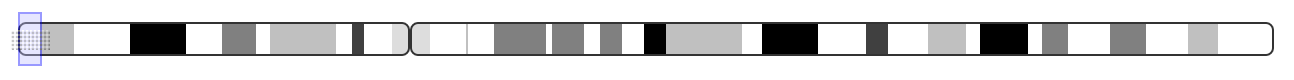
\includegraphics[width=\textwidth]{figures/chromosome.png}
\caption[BioJS component to represent a Chromosome]{BioJS component to represent a Chromosome
\label{fig:biojs_chromosome}}
\end{figure}

Figure \ref{fig:biojs_chromosome} is an snapshot of the BioJS component displaying chromosome 8 from \emph{Homo sapiens}. The information is obtained from the DAS server provided by Ensembl that contains the karyotype information (\url{http://www.ensembl.org/das/Homo_sapiens.NCBI36.karyotype/features?segment=8}). The DAS response is processed using JsDAS, extracting information about the chromosomic location, name and category of each band, which ultimately defines where, what label and which colour will be used to paint the region in the component.

The chromosome is represented in a web page by a composition of HTML div elements, where all the divs are drawn on the same line without any separation between themselves. CSS classes are defined for each of the chromosome categories, for example the style below will be assign to the div that is rendered with a gpos25  category.

\begin{lstlisting}[language=HTML]
.gpos25 {
	background-color: rgb(25%, 25%, 25%);
}
\end{lstlisting}

The border of the bands at both edges of the chromosome and the ones next to the centromere are rounded in order to visually identify these areas (as seen in figure \ref{fig:biojs_chromosome}).

The component broadcast events when the user hovers or clicks over a band, in the examples this is used to display a label or to reposition an area selector over the corresponding bar. This area selector is an utility BioJS component (\url{http://www.ebi.ac.uk/Tools/biojs/registry/Biojs.AreaSelector.html}), that although is not biological related, it can be reused by any component that uses a similar approach to the graphic representation (i.e. HTML elements). Figure \ref{fig:biojs_chromosome} shows the selector over the band that is at the left of the chromosome. The selected region can be manipulated by dragging the edges of the blue area, and every time a new area is marked, events are broadcasted and other BioJS component can react accordingly.

In BioJS 2.0 is recommended to only publish biological related components, therefore we decided to exclude the Area selector component from the BioJS registry. Nonetheless the component was published in npm (\url{https://www.npmjs.com/package/area_selector}) and can be reused by other npm packages including those part of BIoJS
 
\subsubsection{Protein-Protein Interactions Force Layout} \label{subsubsec:ppi_biojs}
The most popular way to visualise networks is known as the node-link metaphor, in which some figures (e.g. circles. squares, images) represent the nodes; and lines connecting them are the links. When the network consists of a short amount of nodes, it is possible to specify the position for all of them, however when the amount of nodes grows, the effort required to position all of them also increases and random location of nodes would probably generates highly congested graphics with overlapping of elements and very cluttered areas.

Different strategies have been defined to automatically organise network representations. We have used the implementation of a force-directed layout included in the D3 library (\url{https://github.com/mbostock/d3/wiki/Force-Layout}) \cite{BOS2011} for the BioJS component that can visualise protein-protein interaction networks in a web native component:  \url{http://www.ebi.ac.uk/Tools/biojs/registry/Biojs.InteractionsD3.html}, \url{http://biojs.io/d/biojs-vis-interactions-d3}.

The force directed layout implemented in D3 follows the simile of attaching springs to all the connected nodes, in this way  two nodes connected pull towards each other, and if a node has several links it is subjected to all the spring forces of its connections at the same time. The algorithm also includes a rejection force between all the nodes, which aims to disperse unconnected nodes and avoid cluttered areas. An optional gravity point can be setup where all the nodes are attracted, this helps to keep the nodes in the visible area. 

The simulation of the movement of the nodes caused by the defined forces is executed by steps. For each step, all the forces affecting a node are used to calculate a new position for it, and this is done for all the nodes. An internal temperature parameter is used to control the speed of change during each step: when the simulation starts the temperature is high and the particles move fast, and with each iteration the network gets closer to an stable position dropping the temperature, and the nodes move slower as a consequence. The use of the temperature parameter also helps to stop completely the simulation when is lower than a predefined value, this with the purpose of avoiding unnecessary CPU use.The simulation might be required to restart when for example new nodes or links are added to the network, in which case the temperature parameter is changed to a high value.

In order to optimise the number of operations required on each step, the D3 implementation includes a data structure called quadtree that creates a hierarchical organisation of the nodes based in their location. This is used when calculating the rejection forces of each node, so instead of considering all the rejection forces, an aggregated value for the nodes in a region can be used.

A quadtree divides the area in quadrants, the root of the tree contains all the nodes and it has four branches. The first branch contains the nodes that are located in the first quadrant of the graphic (i.e. between the top-left corner and the centre of the graphic), the second branch includes the nodes inside the second quadrant, etc. The same division can be recursively calculated for each quadrant.

The decision on how deep in the structure the algorithm should go to calculate the rejection forces is based on the criterium known as Barnes-Hut \cite{BAR1986}. If the quotient between the width of the quadrant \emph{s} and the distance from the node to the centre of the quadrant \emph{d} is less than a threshold value $\theta$, the aggregated force of the quadrant is sufficient and the recursion on the tree can be stopped. 
%The equation is manipulated to avoid the use of square roots and is written into the D3 library as the conditional:

%\begin{lstlisting}[language=java]
%if (dw * dw / theta2 < dn) 
%\end{lstlisting}

An step in the simulation is concluded when all the forces of all the nodes have been use to calculate the new positions of all the nodes. And every time an step concludes, an event called \emph{tick} is broadcasted. Listeners of the event, can then alter the behaviour of the simulation by adding other forces, for instance to contain the nodes in a frame, or to define several gravity points. The event is also useful to trigger changes in the graphic representing the network, and in this way to animate the simulation.

For the BioJS PPI force layout component we used the \emph{tick} event not only to display the simulation but also to  define multiples \emph{foci} of gravity, one for each organism reported as a protein, in this way the proteins that belong the same organism get attracted to the same area.

The representation of the network in the browser has been implemented using SVG. Path elements forming symbols are used to represent proteins of different organisms. We took advantage of the SVG technology by allowing the user to freely zoom and pan around the graphic with popular mouse gestures i.e. scrolling for zooming and dragging for panning, owever, if the user is dragging the mouse over one of the figures representing a protein, only that node gets moved and once the mouse id released, the protein is forced to stay in the position were the user drops it, this action restarts the simulation in  order to find positions for the rest of the proteins in the graphic.

A running example of this component has been published in \url{http://jsfiddle.net/Bvh6k/8/} using JSFiddle (\url{http://jsfiddle.net/}), an online resource that supports the edition and live execution of snippets of Javascript code. Details on the biological entities used in the example can be found in \cite{SAL2014}. Figure \ref{fig:biojs_force} is an snapshot of the visualisation generated by this example. 

\begin{figure}[ht]
\centering
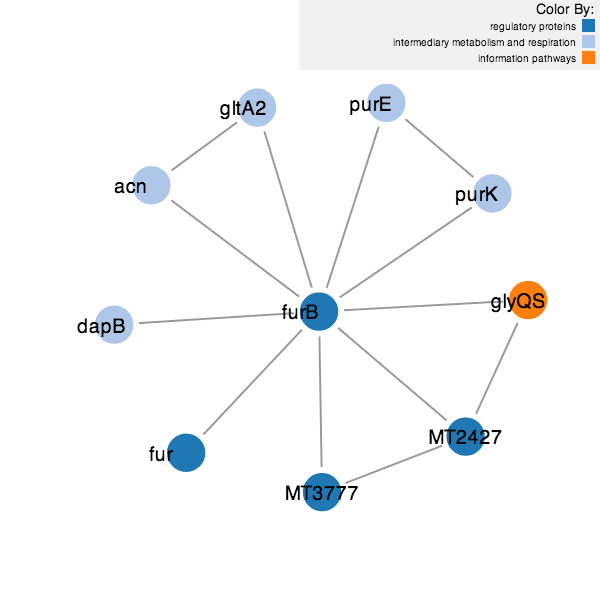
\includegraphics[width=5in]{figures/force.png}
\caption[BioJS component to represent a network using the force-directed layout]{BioJS component to represent a network using the force-directed layout
\label{fig:biojs_force}}
\end{figure}

Besides allowing developers to experiment with the code, the example serve us to explain the use of the component. 

A developer should start by creating an instance of the component:

\begin{lstlisting}[language=java]
var instance = new Biojs.InteractionsD3({
   target: "example"
});
\end{lstlisting}
					
All the proteins in the graphic should then be added. The following example shows how to add the protein with UniProt id O05839 (\url{http://www.uniprot.org/uniprot/O05839}). Note how the organism to which it belongs is included, along with which feature should be used for the label:

\begin{lstlisting}[language=java]
instance.addProtein({
      id: "O05839", organism: "MTB",
      gene_name:"furB",
      typeLegend:"gene_name"});
\end{lstlisting}
					
In the same way, the interactions should be added to the graphic, making sure that the interactions are between proteins that have already been added. For instance:

\begin{lstlisting}[language=java]
instance.addInteraction(
      "O05839", "P0A582",
      {id: "P0A582_P0A582"}); 
\end{lstlisting}
					
Once all the proteins and interactions have been declared, the graphic can be restarted so it reflects the additions:

\begin{lstlisting}[language=java]
instance.restart ();
\end{lstlisting}

The example also includes some instructions for colouring and format. 


\subsubsection{Protein-Protein Interactions Circle Layout} \label{subsubsec:ppi2_biojs}
We have developed another component to display PPI networks that uses the D3 implementation of a circle layout: \url{http://www.ebi.ac.uk/Tools/biojs/registry/Biojs.InteractionsBundleD3.html}. In this layout the proteins are organised in a circle, positioning all the nodes around the centre without favouring any of them, this can help to discover connection patterns around the network (Figure \ref{fig:biojs_circle}). 

The interactions in this visualisation are spline curves which path is defined through the hierarchical edge bundle algorithm \cite{HOL2006}. This algorithm requires the data to be organised in a hierarchy, and in the case of been used in combination of a circle layout, the non-leave nodes of the tree are organised following a radial pattern, where the root of the tree is in the centre, and first level children are located in a circumference around it, the nodes of the following level of the tree are position in a circumference of bigger radius around the root. The same is then done for all the levels of the hierarchy. The nodes in the last level, which are the leaves of the tree, are the only visible ones.

When an interaction between two nodes is drawn, the curve's path will be created using the hierarchy nodes as guidelines. This method highlights the links between two highly connected groups in the hierarchy, because all of those connections will follow a similar inner path, creating the impression of a bundled connection, hence the name of the algorithm.

The hierarchy used for the BioJS component to display PPI network is a two level tree, that simply separates the proteins by organism, which is useful when looking to multi-organism networks such as a host-pathogen scenario. Another case of multi-organisms is discussed in section \ref{sec:orthologs}, where pseudo-interactions were defined to identify a relationship between two orthologs.

\begin{figure}[ht]
\centering
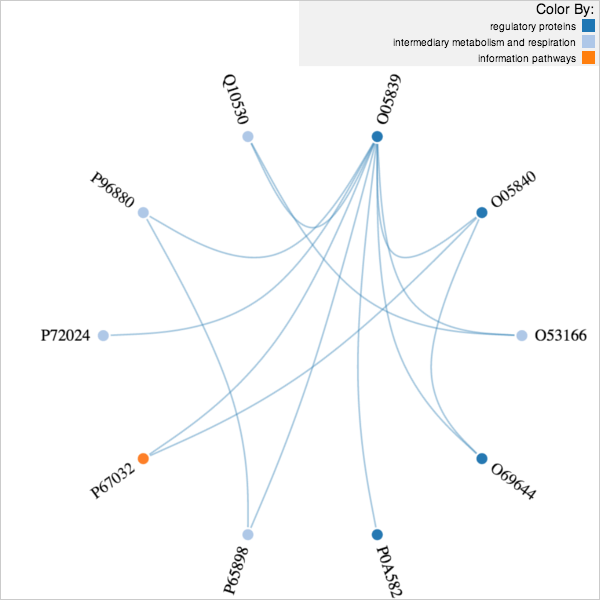
\includegraphics[width=5in]{figures/circle.png}
\caption[BioJS component to represent a network using the circle layout]{BioJS component to represent a network using the circle layout
\label{fig:biojs_circle}}
\end{figure}

Figure \ref{fig:biojs_circle} shows an snapshot of the component displaying the same dataset as the example for the force-layout component, which has been also uploaded as a JsFiddle: \url{http://jsfiddle.net/J4CE7/9/}.

Both components follow the same API (Application Program Interface) and therefore any script developed to display on one layout can be used on the other. The only difference between the APIs is because of methods that help to control the force layout of the first component which do not apply to the Circle layout. Thanks to this, the script to generate a PPI visualization of the same network is very similar in both.  The only difference between the two scripts loaded in JsFiddle is the declaration of the object. Instead of using the object Biojs.InteractionsD3 it uses Biojs.InteractionsBundleD3 and rest of the script is exactly the same.
\begin{lstlisting}[language=java]
var instance = new Biojs.InteractionsBundleD3({
    target: "example",
});
\end{lstlisting}





\subsubsection{Protein-Protein Interactions: Heat Map} \label{subsubsec:ppi3_biojs}
After the publication of \cite{SAL2014} where we described the two components explained in the previous sections, we decided to explore an alternative to visualise PPI interactions. A new BioJS component was developed to visualise the interactions as a matrix of proteins by proteins, similar to the way that some heat maps are used in the processing of microarrays or phylogenetics analysis, but in this case not all the squares of the matrix are filled, only those marking an interaction between two proteins are painted. The component is now in the BioJS 2.0 registry (\url{http://biojs.io/d/biojs-vis-interactions-heatmap-d3}) and the source code is freely available in GitHub (\url{https://github.com/4ndr01d3/biojs-vis-interactions-heatmap-d3}).

This method to visualise PPI networks put the emphasis of the graphic in the interactions rather than in the proteins. And by sorting the matrix and using a correct colouring of the protein labels, for instance based in the functional class, it is possible to find features that other wise aren't evident in a node-link representation because the overlapping of the interaction lines.

Figure \ref{fig:biojs_heatmap} is a snapshot of this component  in which random interactions of 15 fake proteins are displayed. We have included extra functionality in the example to demonstrate the use of some of the methods and events provided in the API of the component. The mouse pointer in the figure is located over the cell that remarks the interaction between \emph{prot\_2} and \emph{prot\_15}, hence the lines crossing over it. We have also clicked on that interaction cell, which triggers an event that displays two panels with the feature information of the interacting proteins. The size of panels and graphic have been optimised for better use the available space on the SVG container.

The interactions in the example have been coloured using a scale between red and green based in the other this proteins are included into the model. This feature can be used to represent any quantifiable value associated with the interaction, for example evidence scores.

\begin{figure}[ht]
\centering
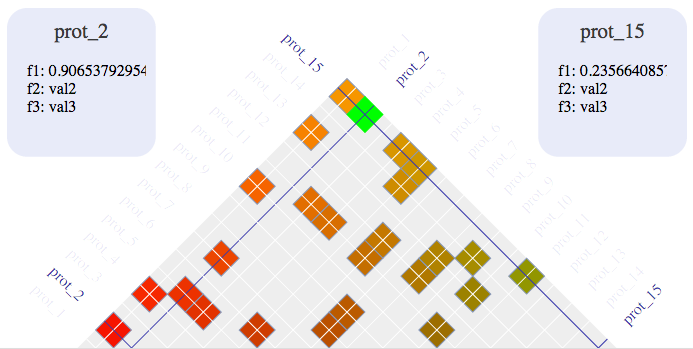
\includegraphics[width=\textwidth]{figures/heatmap.png}
\caption[BioJS component to represent a network using a heat map]{BioJS component to represent a network using a heat map
\label{fig:biojs_heatmap}}
\end{figure}

An interactive example of this component can be accessed directly form the BioJS registry (\url{http://workmen.biojs.net/jsbin/biojs-vis-interactions-heatmap-d3/simple_example}). In this case we are using a different tool called JSBin, which behaves similarly to JsFiddle, the tool used in the examples of the previous components. JSBin has a better support for the inclusion of npm packages and therefore it is easier to use with BioJS 2.0 components.

The component also shares the same API as the previous two PPI visualisation widgets, which makes it easy to alternate the view between the 3 PPI components and in this way offer to the user several options to display their data.


\subsection{Discussion}
We have discussed in the introduction (section \ref{sec:ppi}) the existence of several tools that visualise PPI networks; all of which support variations of a force-directed layout. However by the time we developed the components described in this section, there were not web components to create such visualisations using HTML5 web standards. We are aware now of the existence of the Cytoscape.js project, which offers an alternative based in the HTML5 element canvas and include implementations of not only force-directed layouts but also circle, grid, and others. Nonetheless, we consider that is important to have technology alternatives  for this type of components. If for example, a developer is already using D3 in its web tool, the use of our components can be a better alternative to reduce the network latency created by many dependencies.

\newpage





\section{PINV, a web-based Protein Interaction Network Visualiser }  \label{section:pinv}
Protein-protein interaction data has been used in multiple research scenarios: (i) to browse networks for genes of interest, (ii) to interpret the results of genome-wide genomic screen, (iii) to interpret functional genomics data and (iv) to elucidate disease genes \cite{FRA2013}. In all of them visualisation has play an important role, for instance,  to meaningful navigate around a big network (i and iv), to find clusters of proteins with shared functionalities(iii and iv)  or highlight links that are not evident with other techniques (i and ii).

Multiple projects to visualise PPI networks have been discussed in section \ref{sec:ppi}, however none of them uses the web as their platform and in consequence their collaborative capabilities are limited. 

The potential of community oriented projects built on the web has been exposed in other fields, for example GitHub has become the most popular system to collaborate in open source projects, with more than eight million users and over twenty million repositories by the beginning of 2015 (\url{https://github.com/about/press}), and although the core of it is the git version control software, it is arguably that the web front end is the one who attracts the community to take part of many open source projects.

We have developed PINV, with the goal of bringing this potential into the research of PPI networks. An article describing the project was published in 2014 and is listed as No. \ref{paper:PINV} at the beginning of this chapter. The first author of this publication is Gustavo A. Salazar and the co-authors provided input in line with their roles as collaborators and supervisors. Below we describe PINV in more detail, including its architecture and implementation.

\subsection{Description of the application} \label{section:pinv_gui}

PINV can be accessed in the web via this URL: (\url{http://biosual.cbio.uct.ac.za/pinv.html}). The visitor is presented a menu with four options: Data sets, Load data, Documentation and about. 

The \emph{Data sets} page is the default, here the user can find a list of all the public datasets that have been upload into PINV. We have loaded some public datasets for organisms of our particular interest: \emph{Homo sapiens} (HS), \emph{Mycobacterium leprae} strain TN (MLP), \emph{Mycobacterium smegmatis} strain MC$^2$155, \emph{Mycobacterium tuberculosis} strain CDC1551  (MTB) and a combined dataset of \emph{HS}, \emph{MTB} and the interactions between them. The rest of the datasets on the list have been uploaded by PINV's users. We have included a search functionality in the page where users can include part of the name of the dataset and the list is automatically updated to only include those that match the given text.

The second option in the home page is \emph{Load data}, here a web form is displayed. The required information consist in a unique name for the dataset, a valid email where the user will receive the links to access the dataset, the preference between a public or a protected dataset (difference explained in the next section), and two tab separated files: one for interactions and one for features.

In the interaction file, the first two columns contain the accession numbers of the proteins, and the third column is an aggregate score of the evidence for the reported interaction. Subsequent columns are optional and considered as evidence scores that contributed to the unified value in column 3.
The second file is used to add annotations to the proteins (e.g., gene name). The only required annotation is that of the organism to which the protein belongs; therefore the file should have the protein id in the first column, the organism in the second and any other features in additional columns. The information provided in this file can then be used to manipulate the graphic, for instance to color by functional class or to show a particular label.

The last two options of PINV are \emph{Documentation} and \emph{About} where resources to provide help to the user are included. For example, tutorials, presentations and links to the source code and the original publication.

\begin{figure}[ht]
\centering
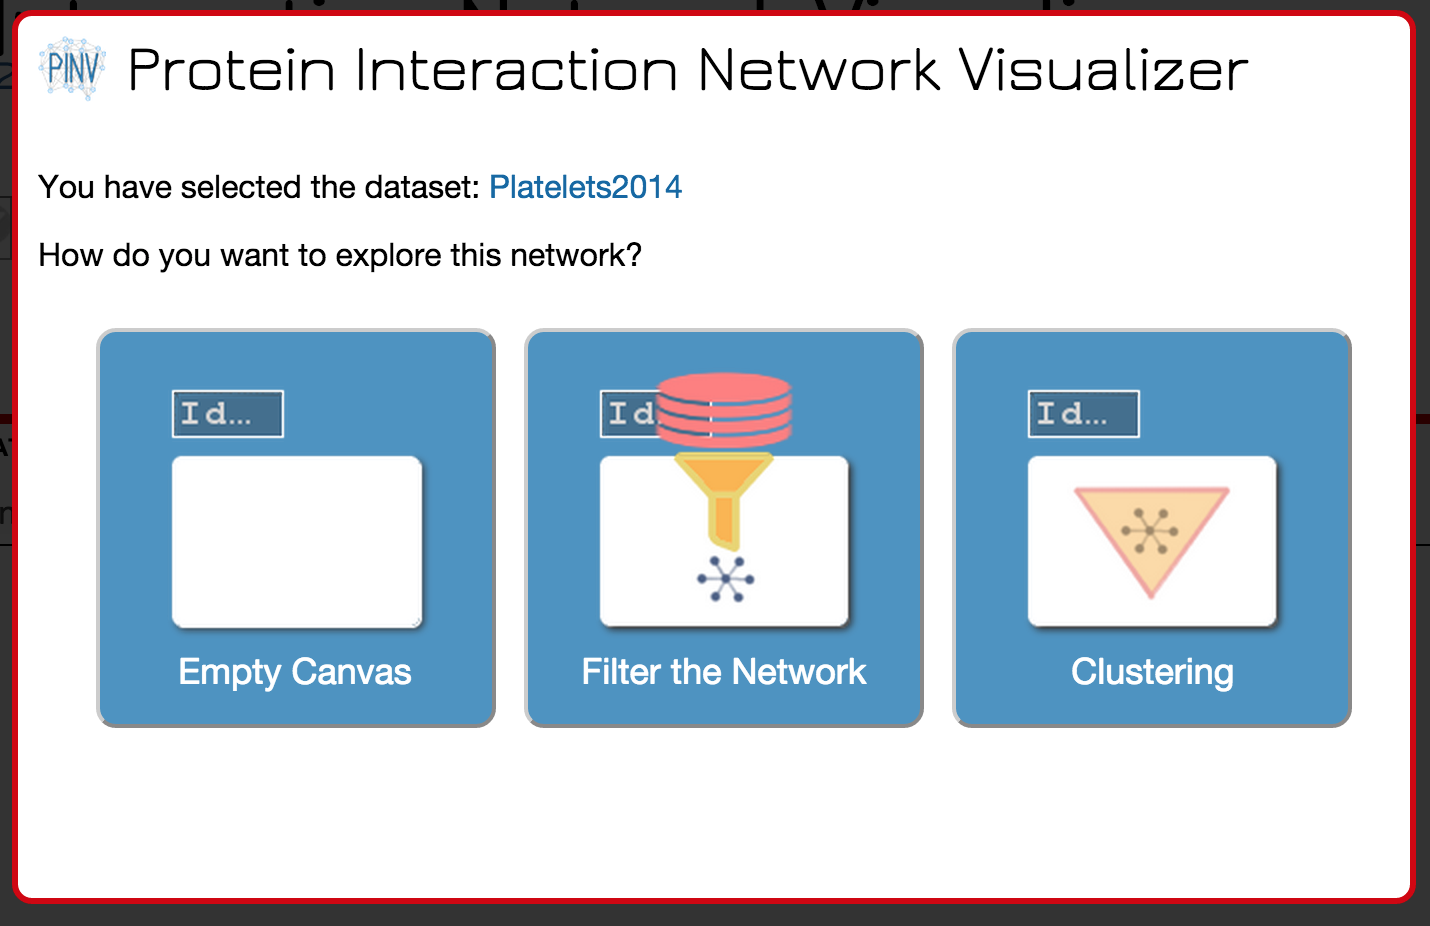
\includegraphics[width=\textwidth]{figures/pinv_wizard.png}
\caption[Wizard menu to select the exploration method in PINV]{Wizard menu to select the exploration method in PINV
\label{fig:pinv_wizard}}
\end{figure}

Once users select a data set from the list or access one from the link sent to their emails, the PINV client is load into the browser (See the client part in section \ref{pinv_architecture}) and then, a popup window(Figure \ref{fig:pinv_wizard}) presenting three options to explore the data is displayed:

\begin{description}
\item[Empty Canvas] 
Using this method the interface displays all the widgets, but no queries had been executed, and therefore the visualisations are empty. The proteins of interest can be selected by inserting comma separated accession numbers. The form has auto-complete capabilities to assist in this process (Figure \ref{fig:pinv}-A). 

The search function has three modes: Normal, Explicit and Recursive. The \emph{Normal} mode returns the queried proteins and all interactions reported in the dataset, while the \emph{Explicit} mode will only display proteins that have been explicitly included in the query list and the interactions between them; the explicit mode will also include all the interactions with the previous results.
The \emph{Recursive} mode combines the previous two, it first gets the target proteins on \emph{Normal} mode, and then for each recovered protein it triggers a query in \emph{Explicit} mode, the outcome of this is that all the interactions between displayed proteins will be shown.

\item[Filter the Network] 
In order to meaningfully visualize protein interactions, it is beneficial to reduce the network to only those proteins of interest through the application of prefilters to the data. This has the simultaneous benefits of increasing the speed of PINV's response time and reducing bandwidth requirements. By using the prefilter tool on PINV, the user can explore the whole content of the network without loading the individual components into the graphic. Figure \ref{fig:pinv_filters} (Left) shows the interface where the user can define certain conditions that the interactions have to fulfil in order to be displayed. The graphic on the left side of Figure \ref{fig:pinv_filters} is dynamically updated, reflecting the size of the subset generated by applying the filters over the whole dataset. For instance, in the graphic the dark blue represents the whole network (796353 interactions), while the light blue is the portion of those that have an evidence score from STRING \cite{FRA2013}. Two more filters were applied to this example (\emph{organism contains tuberculosis} and \emph{description contains Sensor}), the combined use of the filters results in a 103 interaction subnetwork, which is small enough to allow PINV to run smoothly and generates a graphic like that in Figure \ref{fig:pinv_filters} (Right).

\begin{figure}[ht]
\centering
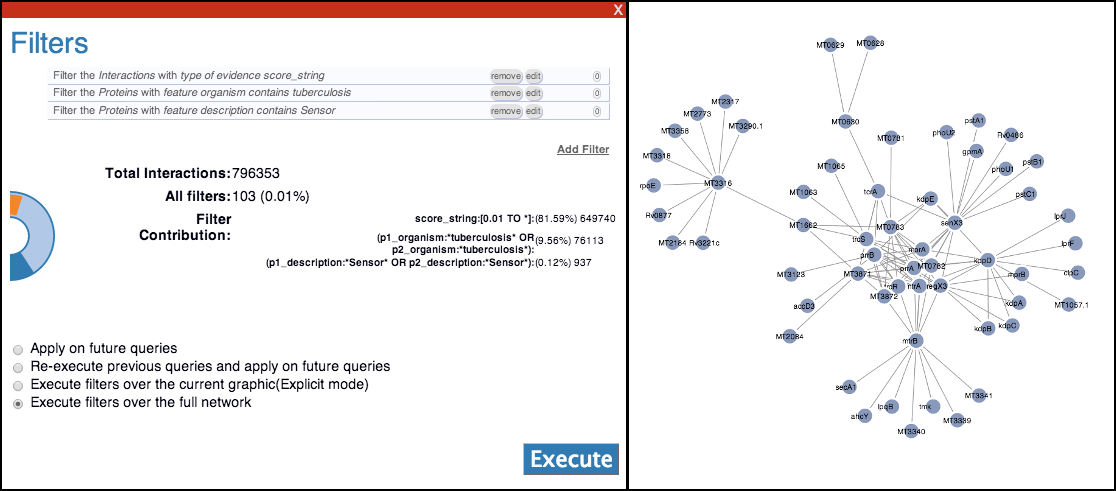
\includegraphics[width=\textwidth]{figures/PinvFilters.png}
\caption[PINV Filters Dialog.]{PINV Filters Dialog. Snapshot of the dialog where the user can explore a dataset by defining filters.
\label{fig:pinv_filters}}
\end{figure}

\item[Clustering] In this mode the whole network is represented by clusters of proteins and interactions between them, the user can then expand the clusters, to explore the network in a top-bottom fashion. A more detailed description of this method is included in section \ref{section:clustering}.
\end{description}

\begin{figure}  
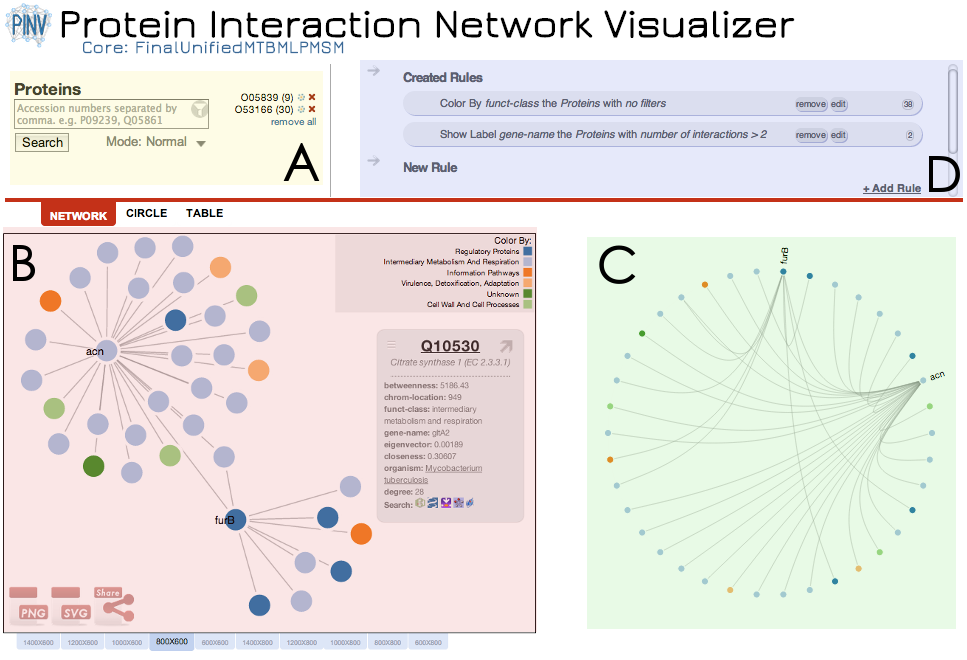
\includegraphics[height=5.7in,angle=90]{figures/pinv.png}
\caption[PINV Snapshot.]{PINV Snapshot. (A) Search Form. (B) Network layout. (C) Circle layout (D) Manipulation by Rules.
\label{fig:pinv}}
\end{figure}

PINV provides four types of visualisation of the data: Network, Circle, Heatmap and Table. The first three types were implemented as BioJS widgets and have been described in section \ref{subsec:biojs_components}. 

Figure \ref{fig:pinv}-B displays a snapshot of the interactions for proteins O53166 and O05839 from the MTB dataset in the Network layout. The network layout allows the re-organization of the proteins through drag and drop mouse gestures, and clicking on a node will display the loaded features that are hyperlinked to relevant public resources in a pop-up window (right side of Figure \ref{fig:pinv}-B).

The second layout organises the proteins in a circle positioning all the nodes around the center without favouring any of them, this can help to discover connection patterns around the network (Figure \ref{fig:pinv}-C). In this view the interactions of a single protein are highlighted when the user hovers over the node. As in the network layout, the proteins are separated to clearly indicate the organism to which they belong; the user can choose to sort the proteins around the circle by any of the protein features.

Figure \ref{fig:pinv_heatmap} displays the same query of figure \ref{fig:pinv} using the heat map component. In this representation the focus is in the interactions, and the proteins are only labels of them. This visualisation offers the possibility to compare the features of the two proteins involved in a interaction.

\begin{figure}[ht]
\centering
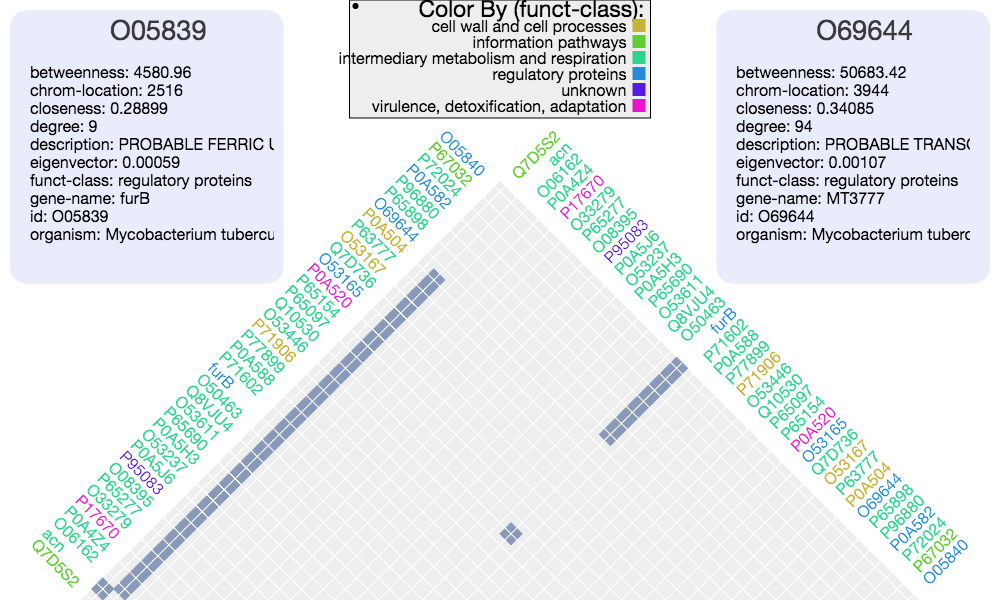
\includegraphics[width=\textwidth]{figures/pinv_heatmap.png}
\caption[PINV Heatmap Visualization.]{PINV Heatmap Visualization of the proteins O53166 and O05839 from the MTB dataset.
\label{fig:pinv_heatmap}}
\end{figure}


Lastly there is the table view where the raw data is displayed and can be reorganised. This is particularly useful for queries that return too many results and require post-filtering to select the proteins of interest.

The visualisation of the layout can be exported at any time into SVG or PNG format, and the data in the table are exportable to a CSV file.

Manipulation of any of the three display options is achieved with a single component (Figure \ref{fig:pinv}-D) that allows the creation of rules. The rationale behind this component is that by specifying a target (protein or interactions), a condition to filter by (e.g., protein with functional class X, interactions with protein Y), and an action (e.g., paint green, show label) it is possible to manipulate a wider set of network elements with less input from the user. For example, Figures \ref{fig:pinv}-B and C show all the proteins painted in different colours depending on their functional class. The legend on the right lists the functional classes used and the corresponding colours in the graphic. A second rule was created in the example to display the gene name at the side of proteins with more than 2 interactions.
Right clicking on a protein in the graphic will open a contextual menu that allows the quick creation of rules that only apply to the selected protein. Users can also colour nodes with quantitative data such as expression values loaded from a third file.

All the actions executed by the user have been saved in order to display the provenance of the visualisation in the form of a list where the user and collaborators can review the steps (and their parameters) taken to reach a particular status of the visualisation. This list can be displayed by clicking on the “Show History” button at the bottom of the page. 

PINV provides an easy way to share the current view: when the user clicks on `share', a unique link is generated. PINV is able to regenerate the status of all the components to re-compose the view whenever the link is used. 
This functionality was developed with the goal of promoting collaboration between users. If for instance, a user finds something of interest in the visualisation, he/she can create the link and send it to a collaborator via mail, instant messaging, etc. The second researcher can not only view but manipulate the visualisation and re-create another link for future discussions. For example, recreations of Figures \ref{fig:pinv_filters} and \ref{fig:pinv} can be explored in PINV by following the URLs \url{http://biosual.cbio.uct.ac.za/pinViewer.html?status=paperF} and \url{http://biosual.cbio.uct.ac.za/pinViewer.html?status=paper00} respectively.

The sharing option also provides an HTML snippet that can be used embed the view in a web page, making it easier for the researcher to include their visualisations on web documents in the same way that maps, videos and other kinds of multimedia are included in blog posts. It is hoped that researchers will use this to embed PINV graphics in pages that discuss the results of their own network research.




\subsection{Architecture} \label{pinv_architecture}
PINV has been designed to follow a classic client-server architecture, in which the client is in charge of the interaction with the user and the generation of the visualisations, based on asynchronous calls to recover data on demand. The server has been optimised to provide rapid responses through a REST interface, whilst the client follows a modular architecture that makes it easy to extend and adapt. 


\subsubsection{Server}
The server side of PINV has been developed using the web framework for Python called CherryPy (\url{http://www.cherrypy.org/}) and the PPI data is indexed and stored in a Solr search engine server \cite{KUC2013} in order to perform rapid queries, resulting in quicker response times than through querying of a relational database

PINV's client never interacts directly with the Solr instance, instead all communications are tunnelled by the CherryPy component, this with the purpose of prevent the access to resources and functionalities to unauthorised users. For example, the REST services of Solr includes a method to delete a core, which is the term used in Solr to describe the dataset and its controllers. We filtered out such calls and any other administrative functionalities that can harm the data of other users.

The main functionality of the server is to allow the upload of the PPI data from simple tab separated files into a Solr core. When uploading data, the user can choose between two modes of privacy: public and protected. A dataset in public mode will be listed on PINV’s website and accessible to anyone. This brings visibility to the data and promotes collaboration between researchers. On the other hand, protected mode ensures that only users with a valid link can retrieve information from the data set; the link includes a unique key that is sent to the uploader so he can distribute the link as he wishes. In this way the collaborative features of PINV are still functional between the holders of the link.

The authorisation to a protected core is another function managed by the CherryPy server. The access to any information of a protected core is restricted to the inclusion of the key into the request. When data is upload to PINV in protected mode, an email including links with the key in it will be sent to the user. A similar email is also sent to owners of public datasets, which include links to restricted administrative functions such as deleting the core.

Another feature carried out by PINV's implementation of the CherryPy server is to allow the storage and posterior retrieval of the files that contain the status the different widgets, which is the key element in the generation of links to share or embed a visualisation created in the tool. When the user clicks on the share button, the client compile the state of all its widgets in a single configuration file, including the current dataset, queries executed, graphic manipulation rules, etc.This file is sent to the server, where is stored and a unique identifier is assigned to it, the ID is then returned to the client which uses it to generate the URL and the HTML code to embed PINV in another page. When the link is used, the PINV client loads normally (See following section), but in addition the status email is recovered from the server and used to reload all the configurations and regenerate the visualisation.

Following the principle of making PINV an open source project, we have published the repository in GitHub (\url{https://github.com/4ndr01d3/pinv-server}) that includes the CherryPy logic, a Solr installation that has been configured to be used in PINV, an example configuration to use apache to redirect any Solr query into CherryPY, and documentation or all these components.

\subsubsection{Client}
When the user selects a dataset from PINV's home page, the main application gets loaded into the client, which initially means that two resources get retrieved from the server: a bundled javascript that contains PINV's scripts and all the widget files, and a similarly bundled CSS style file. These files are built on demand in the server by a PHP script that checks the configurations included in JSON file that is store in the server. 

This schema allows modularity in PINV so when new widgets are developed, the core of the application remains the same and only the configuration files needs to be modified. It is also possible to have several configuration files to create instances of PINV with different widgets, for example the home page of the project executes the same routines, but includes different widgets to display the list of available datasets, the forms to upload data and the documentation of the system.

\begin{figure}
\centering
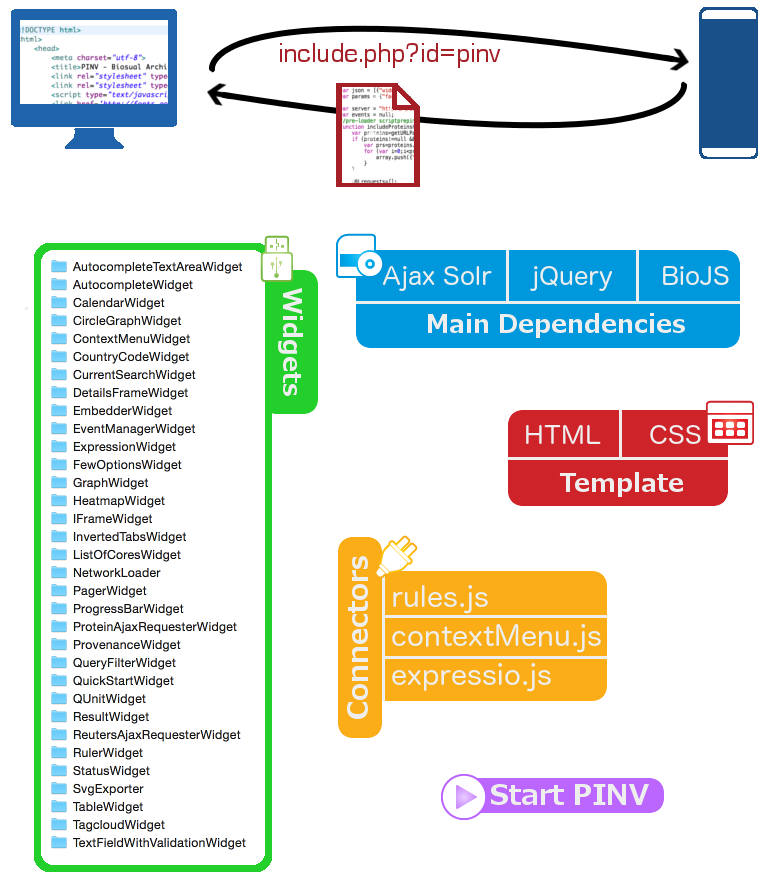
\includegraphics[width=\textwidth]{figures/include_php.png}
\caption[Files to be included by the PHP script of PINV]{Files to be included by the PHP script of PINV
\label{fig:pinv_include}}
\end{figure}

Figure \ref{fig:pinv_include} shows all the components that provide the whole client logic of PINV. As mentioned above, these components are compiled in a singled javascript file by a PHP script. Having a single file reduces the time of loading because it requires only one HTTP transaction. 
\begin{description}
\item[Main Dependencies] 
There are three main dependencies included in PINV: jQuery, AjaxSolr and BioJS. 

PINV uses jQuery (\url{https://jquery.com/}) in several ways, for instance to manipulate data object model DOM, which is the data structure that contains the HTML elements in web browser; this can be done without jQuery, but its syntax facilitates the process; jQuery is also extensible via plugins and PINV uses several of this extensions (e.g. draggable components, auto complete features, etc.).

The second general dependency is AjaxSolr (\url{https://github.com/evolvingweb/ajax-solr}) a library that serves as the interface with the Solr server that contains the PPI network data. AjaxSolr architecture follows a Model-View-Controller MVC pattern that has been adapted to the interaction with a Solr server: the model is based in the structure of the documents retrieved from the server; widgets are registered to the AjaxSolr core, which acts as the controller, notifying the widgets about the actions and results of interacting with the server. Widgets are in charge of generating the views, because they can include methods to react according to each notification, for example to display the results of a query once the core triggers an \emph{afterRequest} event. 

PINV reuses this strategy, and each of the components that form this application have been developed as AjaxSolr widgets, so they can get notified of each interaction with the server, some of the widgets use the core to execute new requests, while other wait for responses to generate views.

The main class of BioJS 1.0 is the last general dependency included in the compiled file. The visualisation widgets included in PINV have been implemented following the BioJS standards. Each of the components described in section \ref{subsec:biojs_components} are used in PINV: the logic related with PINV was written as an AjaxSolr widget, but all the visualisation features were kept as a separated BioJS component. All of these components inherit from the BioJS class added in this step.

\item[HTML Template]
After the dependencies have been included, the script proceeds to extract the information about the HTML template from the configuration file. The template is a HTML piece of code that works as layout for the components, specifying divs or other container elements where the widgets can be included in a later stage. In this step the PHP script creates a variable in the javascript code containing the selected template, and then a piece of executable is added to inject the template into the DOM of web page.

\item[Widgets]
As mentioned before a widget in PINV follows the schema defined in AjaxSolr, however we extended this concept in order to include other resources related with each widget. In the server each widget has its own folder, which should contain a configuration file called widget.json. The PHP reads  this file in order to extract the paths of each of these resources: JavaScript dependencies, CSS dependencies, HTML, CSS and the JavaScript widget. Only the JavaScript file is required, all the other resources are optional. 

The code below is the configuration file used to describe the widget that displays the network using the force-directed layout using the BioJS component described in section \ref{subsec:biojs_components}. The \emph{GraphWidget.js} file defines the widget as a class that inherits from \emph{AjaxSolr.AbstractWidget} and implements the methods to initialise the widget and process all the interactions with the server; The widgets uses the BioJS component \emph{Biojs.InteractionsD3.js} to visualise the interactions, which in times uses the implementation of the force-directed layout included in the D3 library (\emph{d3.min.js}). The HTML in \emph{GraphWidget.html} is limited to the definition of a div element where the component will be included.

\begin{lstlisting}[language=java]
{
    "name": "Interaction network",
    "description": "A network graph using D3",
    "dependencies":["d3.min.js","Biojs.InteractionsD3.js"],
    "js": "GraphWidget.js",
    "html": "GraphWidget.html",
    "css": "GraphWidget.css"
} 
\end{lstlisting}
The current version of PINV includes widgets that facilitate the search in the server by ID(\emph{AutocompleteTextAreaWidget}), to filter the query using the protein features (\emph{QueryFilterWidget}), to visualise the interactions using a force-directed layout (\emph{GraphWidget}), a circle layout (\emph{CircleGraphWidget}) and a heat map graphic(\emph{HeatmapWidget}). This visualisations can be manipulated by other widgets, for instance by creating rules to define colour or size  depending on the protein features (\emph{RulerWidget}), or by using expression data to paint the proteins on a corresponding colour scale (\emph{ExpressionWidget}). There are other widgets that were created to provide some GUI features, such as the tabs to select the visualisation method (\emph{InvertedTabsWidget}) or a floating window that can display the features of a selected protein or interaction (\emph{DetailsFrameWidget}).

All the widgets were developed to be able to be executed independently. This means that the whole architecture can be used for a different application, and if the widget applies then it can be used there, for instance the autocomplete text area widget is not attached to protein protein interactions data, and therefore it can be used to generate queries by ID in any other configuration of the system.

\item[Widget Connectors]
In order to keep the widgets reusable, we have separated the logic of their interactions in separate files. The widgets implement the triggering using the common event handler included in BioJS 1.0, however the listeners of the event are not declared in the widget itself, but in the connector files. In this way two  configurations of the system can operate differently based on the same event, but still using the same widget. 

Consider for instance, two configurations of PINV: in the current version there is a tab widget that allows to select which visualisation method is going to be used; alternatively, we can have a configuration were all the visualisation methods are displayed simultaneously. In the first scenario there is not need of communication between the visualisation widgets, while in the second, it is desirable that a click in the symbol that represents a protein in one widget, triggers a reaction in the correspondent elements of the other widgets. 

PINV architecture support this two behaviours without requiring changes in the files that define a widget, but instead including this type logic in the \emph{Widget Connectors} files. The three files that the current version includes are supporting the events generated by: the rule definer widget (\emph{ruleExecuter.js}), the context menu that get displayed when a right click is done over a protein (\emph{contextMenuFunctions.js}) and the widget that processes the expression files  (\emph{expressionExecuter.js}).

These files are only necessary when the interconnection between widgets requires some logic, for example to filter the visible components based on the defined rule, or to interpolate an RGB value based on the limits and colours selected by the user. For other events where the interaction between triggered and listener is more direct, can be simply reported in the configuration file, for example when a click in protein X in a widget, triggers the method \emph(highlightProtein()) in another widget.

\item[Starting logic]
All the files included until this moment are either class definitions or injections of HTML to build the layout of the page, it is only at this stage of the file where the routines to execute all this components are added. 

As explained before, the logic of operation follows the same strategy than AjaxSolr, and therefore the main part of this logic is to instantiate this class and to register all the widgets that are being used.

The configuration file supports the inclusion of a preloaded file, in case there is some logic out of the widgets that needs to be executed previous to the initialisation of widgets. Currently this is used to retrieve the schema of the dataset that a user has selected because each dataset can have different protein features, and this information is used for some widgets, for example the ruler needs to know this feature names in order to build the forms where the user build the rules.

Similarly there is the possibility of including a post loader script, however the current configuration of PINV doesn't make use of this option.
\end{description}


\subsection{Comparison with Similar Tools}
Most interactive online visualization tools only allow the viewing of networks that are preloaded, meaning that the user cannot view a network he/she has generated.

The online version of Graphle \cite{HUT2009} is limited to graphs generated by bioPIXIE in yeast, MEFIT in \emph{E. coli}, or HEFalMp for human data. STRING \cite{FRA2013}, a database for known and predicted protein-protein interactions, and STITCH \cite{KUH2008}, its sister project for chemical-protein interactions, integrate interaction information from various sources in addition to in-house predictions. Both projects use the same library to display their data. However, the network visualized in both databases is barely customizable. The public implementation of VisANT \cite{HU2013}, a web-based  (via Java Applets) workbench for the integrative analysis of biological networks, is based on the Predictome database.  
PINV on the other hand, allows the user to view preloaded data but also to load their own data.

Another alternative is Cytoscape Web \cite{LOP2010}. However, the fact that its introduction tutorial (\url{http://cytoscapeweb.cytoscape.org/tutorial}) requires its users to code in JavaScript indicates that this tool is mainly intended for developers to display networks on the web, not for the scientist who has a network to visualize. In this regard, Cytoscape Web was considered as an alternative to D3 for our background technology to generate the graphics as it is closer to the biological concepts tied to this tool. Unfortunately Cytoscape Web uses Adobe Flash for the generation of the graphics, which goes against our objective of providing a native web application (i.e. developed using recent web standards). 

We also compared PINV with the stand-alone version of Cytoscape by using the network in the biological example mentioned in the following section. The original network contains all interactions from the three organisms and the orthologs with a total of 165,000 interactions. 
The performance of Cytoscape notably exceeded PINV when dealing with a network of this size. Moreover, there are considerably more manipulation options in Cytoscape than the ones currently provided by PINV. However, Cytoscape and its many plugins need to be installed by the user and any collaborator sharing the results.

We are aware that PINV will also struggle to display the 165,000 interactions of the network. However, the strategy of only visualizing by request and the use of prefilters  allows the user to navigate the network by limiting the graphic to the interactions of interest. In contrast Cytoscape web does not provide tools to explore a large dataset and requires the use of the stand-alone application (or other software) in order to filter and create a subnetwork.



%\subsection{Implementation}
%\subsection{Use Cases}

\subsection{Spatial Clustering} \label{section:clustering}
A poster presenting the first version of PINV was exposed at the South African conference in bioinformatics in September 2012, which we consider as the release date of the tool. Many tools have been included since those early days: the pre-filters, the different modes to query, the heat map view, the sharing capabilities and many small improvements and bug fixings, which we hope have contributed in creating a better software product.

A constant challenge during this time has been the scalability of the visualisations, which is not a particular problem of PINV but is common among any tools for network visualisations. This, however is stressed more in PINV because it is a web tool, and the resources available for this visualisation are limited to the ones available in the browser where is been displayed. Moreover, the dynamic representation and the direct manipulation options offered in the tool required dedicated resources for each element in the graphic.

Given the limitations imposed by the underlying technology, the larger the network to be displayed, the slower the performance of PINV. During an in-house test, PINV performed well with subnetworks of up to a thousand interactions, and thereafter performance decreases proportionally to the number of added proteins/interactions. Note that this is highly dependent on the specifications of the users computer. 

In order to overcome this difficulties we have developed an algorithm for clustering that uses the positions that a force-directed layout provides. This with the purpose of offering if not a complete view of a network, at least an approximation of it.

\subsubsection{High level algorithm}
The idea behind the algorithm is simple: highly connected nodes get attracted to each other when imposing a force-directed layout, simultaneously, the rejection forces between nodes, makes that not so connected groups get spread over the graphic area. This creates visual clusters in the graphic. The idea is that instead of creating all the graphic elements representing the nodes and connection of the network, we only display cluster elements that symbolise the group.

The following pseudocode shows the logic of the algorithm. Given a network represented by a two arrays: nodes and links, we apply the force directed layout algorithm to obtain coordinate positions for each element, then we generate cluster elements based on those coordinates (a discussion to the creation of such clusters can be found later in this section). Inner connections are ignored (line 9) because they won't be displayed and interactions with elements out of the cluster are group;  and outer connection will be group.

When painting the network, we can make the size of each cluster to be proportional to the number of nodes that is representing and the thickness of the line between two clusters to represent the number of connections in between them.
\newpage
\begin{lstlisting}[language=java]%,float,floatplacement=H]
nodes =[...]	//Array of the nodes in the network
links = [...]	//Array of the links in between nodes
force_directed_layout(nodes,links) 
clusters = create_clusters(nodes)
cluster_links=[]
foreach link in links {
	cluster_source	= get_cluster(link.source,clusters)
	cluster_target	= get_cluster(link.target,clusters)
	if (cluster_source != cluster_target){
		//try to get an existing link between the clusters
		cluster_link = getLink(cluster_links,cluster_source,cluster_target) 
		if (cluster_link == null) {
			// if there is not link, create one
			cluster_links.append( {
				source:cluster_source, 
				target:cluster_target, 
				number_of_links:1
			})
		} else {
			// if there is an existing link, increment the number of links between the clusters
			cluster_link.number_of_links = cluster_link.number_of_links +1
		}
	}
}
paint_network(clusters,cluster_links)
\end{lstlisting}

Figure \ref{fig:spatial_clustring} shows an example of executing the algorithm. The left side (a) is a node link representation organised through a force-directed layout, the network uses a dataset that reports the co-ocurrence of characters in the novel \emph{Les Miserables}; we have chosen this dataset because it has been used in several examples for network representation in different software tools such as Cytoscape and the D3 library. Figure \ref{fig:spatial_clustring} (b) shows nodes in beige colour representing the created clusters. A interactive execution of this example can be seen in this URL: \url{http://bl.ocks.org/4ndr01d3/2686646672a92aa89a0e}. 

Although the clusters are not perfectly identifying the predefined groups in the dataset, the overall shape of the network is conserved and it is easy to identify  dense areas and highly connected clusters. Future work can be done in representing the cluster in a way where they represent its content, for example creating pie charts to show the contributions of different groups.

\begin{figure}[ht]
\centering
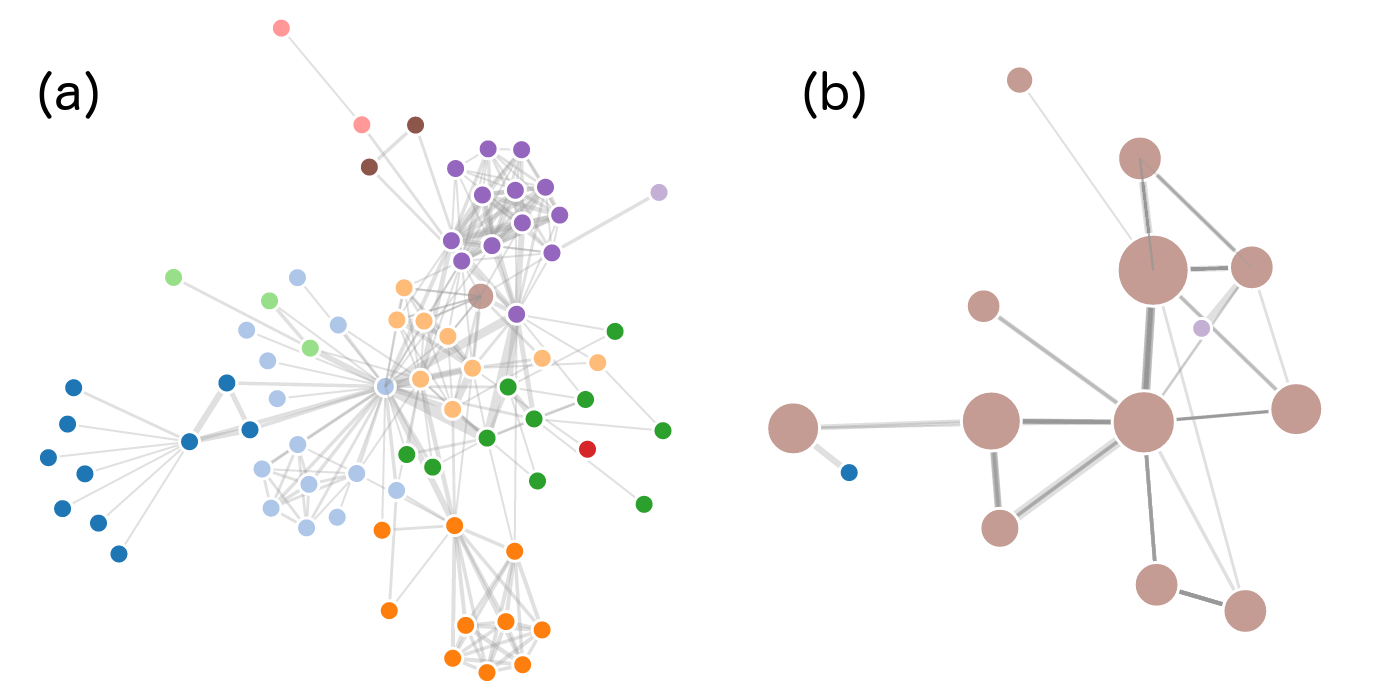
\includegraphics[width=\textwidth]{figures/spatial_clustring.png}
\caption[Spatial Clustering Example.]{Spatial Clustering Example. (a) A networks organised by force-directed layout. (b) A cluster representation of network (a)
\label{fig:spatial_clustring}}
\end{figure}

\subsubsection{Clustering with quadtrees}
The creation of the clusters can be achieved by executing any geometric clustering algorithm, such as k-means. The only restriction is it should use the geometric distance using the coordinates obtained with the force-directed layout, because in this case we are interested in clustering by the position in the graphic and not based in the similarities of the node's features.

However, we decided to create the clusters in an alternative way, inspired in the optimisation of the force-directed layout implemented in the D3 library. Which as discussed in section \ref{subsubsec:ppi_biojs}, uses an structure called quadtree to represent and group the nodes based in its location in the graphic.
 
Figure \ref{fig:quadtree} serve us to explain the construction of a quadtree. In the left side there is an area where points have been randomly located, the algorithm divides the area in four equally sized quadrants, such as the area in light blue representing the bottom-right quadrant. A data structure is created to include the points covered in each of the quadrants. If a quadrant has more than one point, the logic is repeated recursively, saving the results in the same data structure, which creates a tree where all the leaves contain a single point. 

\begin{figure}[ht]
\centering
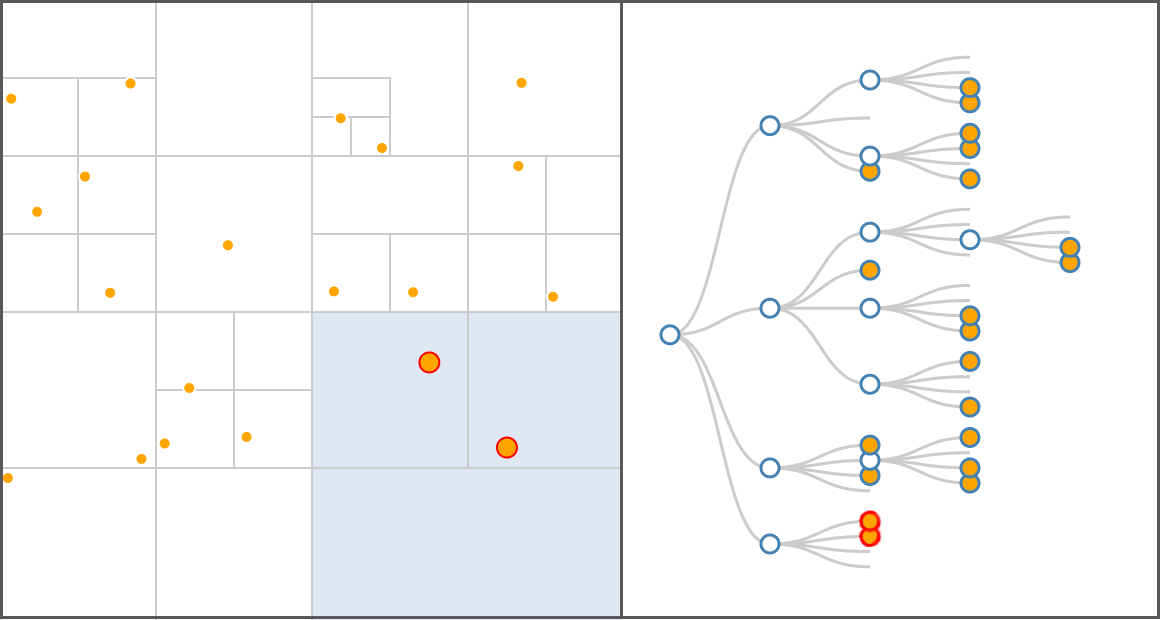
\includegraphics[width=\textwidth]{figures/quadtree.png}
\caption[Quadtree representation of nodes in graphic.]{Quadtree representation of nodes in graphic. 
\label{fig:quadtree}}
\end{figure}

The tree in the right side of figure \ref{fig:quadtree} is the quadtree of the points in the left side. For instance the two points with red border are part of the bottom right quadtree(light blue area) which correspond to the four branch from the root of the tree in the left. Posterior partition shows the nodes in the sub-division top-left and top-right of the graphic, represented in branches 1 and 2 of the subtree.

This data structure has been used to optimise multiple area related algorithms, for example, to detect the collision between bodies: if a body is exclusively located in one quadrant, there is no need to verify for collisions with bodies in other quadrants, this is applied recursively through sub-quadrants, reducing the number of comparisons.

An animation that constructs the tree dynamically can be seen in this URL: \url{http://bl.ocks.org/4ndr01d3/727175afbdc58c3626b8}.

We have used the quadtree structure to define groups of nodes, and provide a way to explore a complex network on a top-bottom approach. The highest level of such representation contains four clusters, one for each quadrant, and the position of a representative element will be calculated as the average of the node positions in that quadrant. The user of such visualisation can choose the level of detail of the graphic representation, which gets interpreted as how deep in the quadtree should the algorithm go.

\subsubsection{Spatial Clustering in PINV}
We have implemented this algorithm in PINV in two different ways: one to be executed with the currently displayed graphic and one to represent a whole dataset.

\begin{description}
\item[On the current graphic]
Executing this algorithm with the current graphic is a task that can be completely achieved in the client side. We used the coordinates of the nodes in the graphic, which have been already calculated with the GraphNetwork widget in PINV that uses the D3 implementation of the force-directed layout. 

We have added a button with the label ``Cluster'' above the graphic that once activated runs the algorithm as shown in figure \ref{fig:local_cluster}, clusters are drawn with grey triangles with red border and its size is proportional to the number of elements that they are representing. When the clustering mode is active an slider is visible at the side of the ``Cluster'' button, allowing the user to select the strength of the clustering, which in other words selects the exploring depth  in the quadtree.

\begin{figure}[ht]
\centering
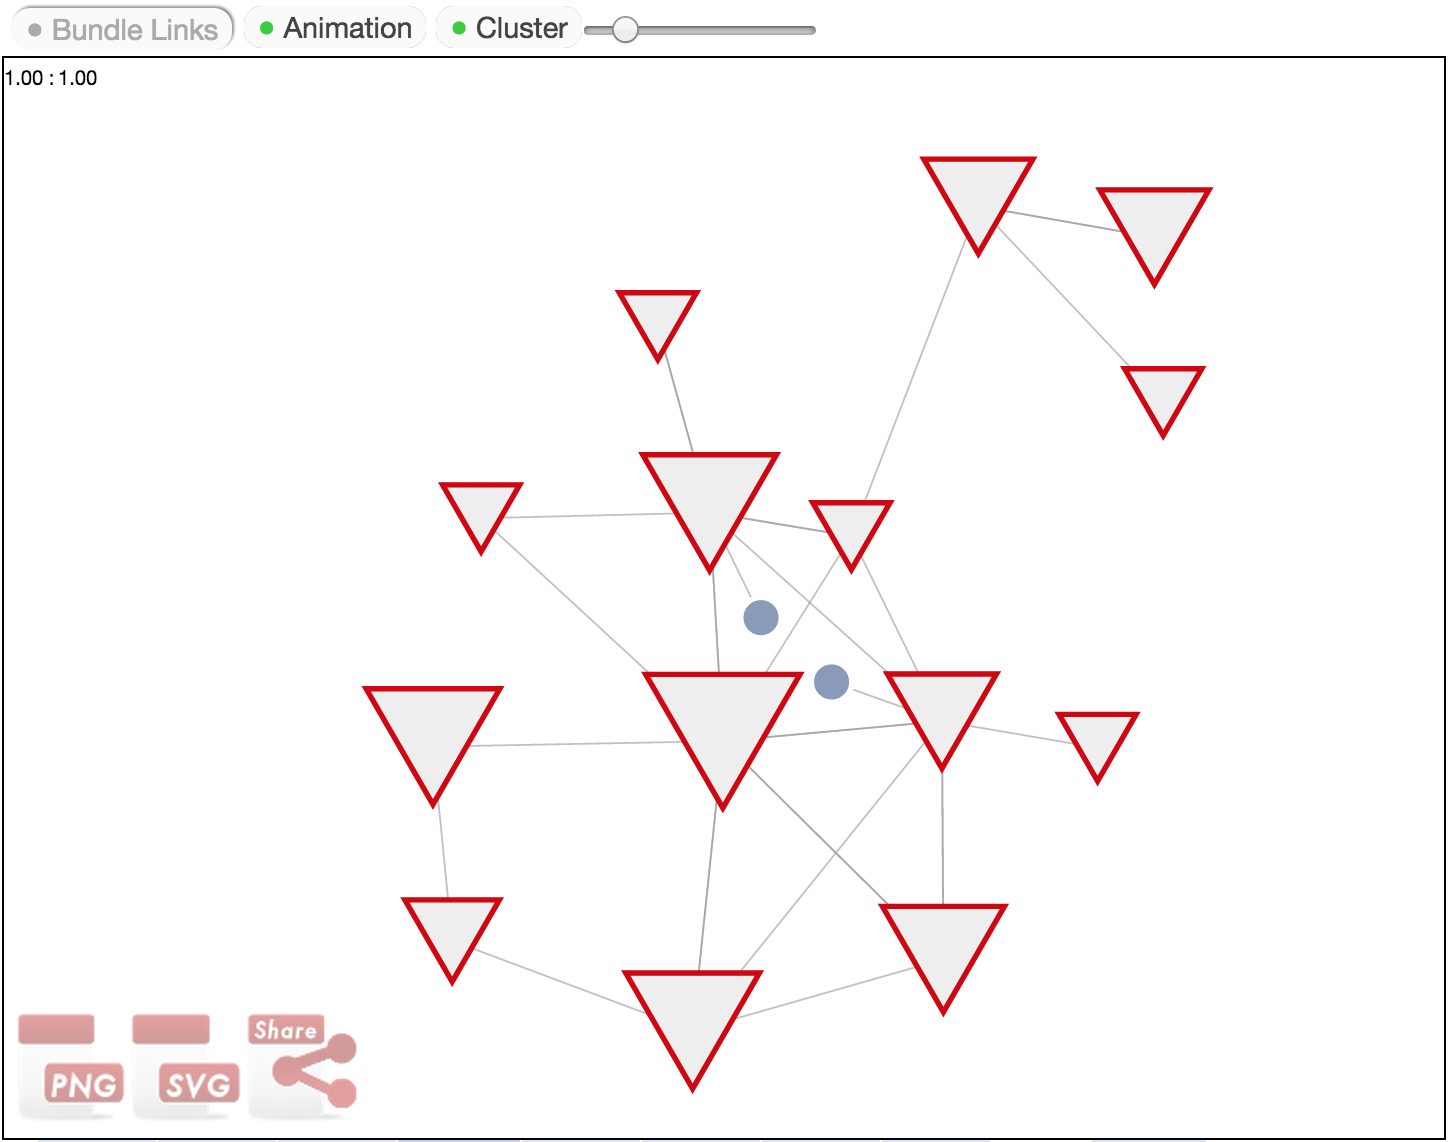
\includegraphics[width=\textwidth]{figures/local_cluster.png}
\caption[Clustering the current graphic.]{Clustering the current graphic. Triangles are elements representing a group of nodes, where its size is proportional to the number of elements.
\label{fig:local_cluster}}
\end{figure}

If a leaf is reached in the tree before reaching the desired depth, it will be represented as a protein and not a cluster. Which is why the figure \ref{fig:local_cluster} has some circles interacting with a cluster.

\item[On the whole dataset]
To be able to calculate a quadtree we required the positions of all the nodes to include. Therefore, either the PINV client requests the whole dataset from the server or the quadtree is calculated in the server. With the first option we could reused the implementation above, but the time required to do all the HTTP transactions to download all the interactions is a problem, however the bigger issue is the performance limitations of the browser.

Therefore we decided to generate the quarter in the server, which implied to implementf both force-directed layout and quadtrees into Python, the language used in our server. The implementation was simply a migration of the JavaScript code in the D3 library, with minor changes to adapted in to Python.

Now every time a new dataset get uploaded in to the PINV server, we execute the force-directed simulation, to obtain coordinates of an imaginary area that can contain all the proteins, using those coordinates we generate a quadtree, and save the interactions between clusters of the first seven levels.

When a user selects a dataset to explore in PINV a menu (Figure \ref{fig:pinv_wizard}) to select the exploration mode is displayed as discussed in section \ref{section:pinv_gui}. If the user chooses the third option \emph{Clustering} PINV queries the server to recover the clusters of level 3, and therefore the graphic will contain up to 64 clusters, which is a number of elements that can be easily handled by the client, but more importantly it is a number graphic that it is more understandable by the user.

\begin{figure}[ht]
\centering
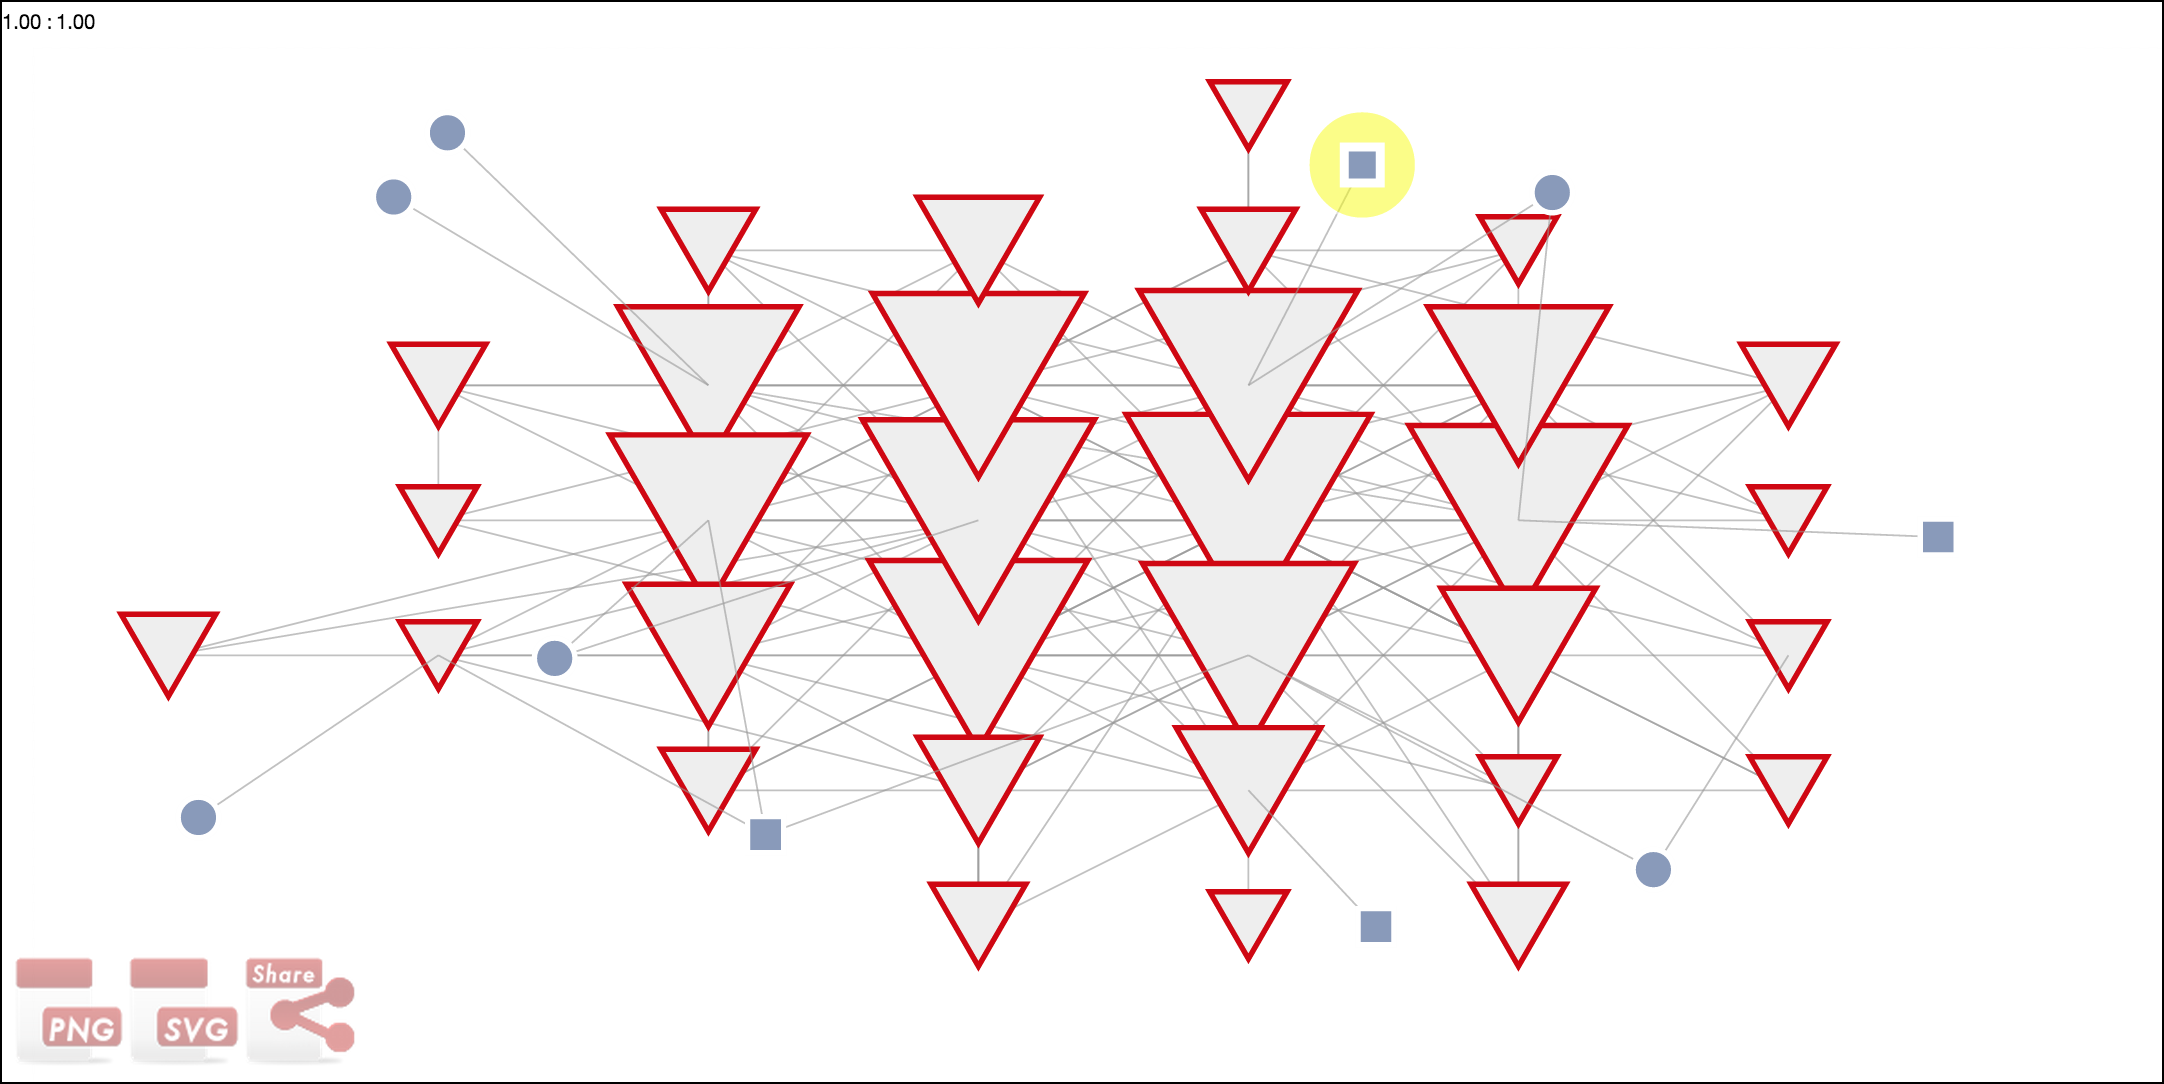
\includegraphics[width=\textwidth]{figures/dataset_cluster.png}
\caption[Clustering the whole dataset.]{Clustering the whole dataset. Cluster representation of the dataset Platelets2014.
\label{fig:dataset_cluster}}
\end{figure}

Figure \ref{fig:dataset_cluster} is the result of visualising the cluster representation of the Platelets2014 dataset. The user can explore the content of a cluster by selecting it, and the list of proteins is displayed in the popup widget for details. Alternatively, the user can double click on a cluster and PINV will request a deeper level of that specific cluster which in turn will be reflected by replacing that cluster by its four children in the quadtree.


\end{description}
\section{Discussion}
PINV is an open source, native web application that uses the latest generation of web technologies to offer an interactive view of protein-protein interactions which is easily accessible from any modern browser. PINV enables researchers to explore their data using different methods and the visualization can be manipulated to highlight the proteins or interactions of interest. The resulting graphic can be exported to common graphic formats, shared via URL or embedded in third-party pages, features that make it suitable for publication, sharing and collaboration activities.

We consider PINV to be a unique tool for visualization and exploration of PPI networks, not only in terms of the technology used (HTML5) but also because today's research requires collaborative efforts to process data. PINV offers an intuitive way to visualize, share and publish PPI data without the need to install any extra software (besides a web browser) and/or third party components such as Flash or Java.

The proposed method to explore whole datasets using an spatial clustering algorithm is not a complete representation of the real network, and we are aware of several implications of the implementation decisions, for example, that the partition by quadtrees can split clusters well defined that other methods can detect easily. However we consider that the use of quadtrees, gives a partial solution that is efficient and allows an easy way to explore a whole dataset form top to bottom.

